%\newcommand{\urlrref}{http://bmw.byuimath.com/dokuwiki/doku.php?id=rref\_calculator}
\newcommand{\onlinetext}{https://content.byui.edu/file/c2f91762-7a1e-4d0b-a1ae-8d5f5f548e17/1/341-Book.pdf}
\newcommand{\urllineartransformationsinplane}{http://bmw.byuimath.com/dokuwiki/doku.php?id=2d\_linear\_transformations}

After completing this chapter, you should be able to:

\begin{enumerate}
\item Explain the connection between vector fields and their corresponding eigenvalues and eigenvectors. Use this knowledge to apply the second derivative test and explore systems of ODEs at equilibrium points.
\item Show how to solve various problems relating to conservation laws (such as stoichiometry, Kirchoff's electrical laws, Markov Processes, etc.) by finding the kernel of a matrix.
\item Use Cramer's rule to solve systems, and explain when you would choose Cramer's rule over row reduction.
\item Find interpolating polynomials, and use the transpose to solve the least squares regression problem.
\item Appropriate apply the words span, basis, vector space, dimension, eigenspace\skipnow{, and linear transformation}.
\end{enumerate}


\newcommand{\ideacon}{Conservation Laws through Eigenvectors and Kernels}
\newcommand{\ideanon}{Nonconservative Eigenvector Problems}
\newcommand{\ideapro}{Projections and Linear Regression}
\newcommand{\idealin}{Visualizing Linear Transformations between Vector Spaces}







\mysubsection{\ideanon}




Vector fields and eigenvalues provide us with precisely the key information needed to locate maximums, minimums, and saddles for functions of the form $z=f(x,y)$. 

\begin{problem}
\marginpar{
Here's a plot of several level curves of $f(x,y)=x^2+4xy-4x+y^2+6y$ and its gradient. In one direction the gradient is pulling things towards the origin.  In another direction, the gradient is pushing things away from the origin.

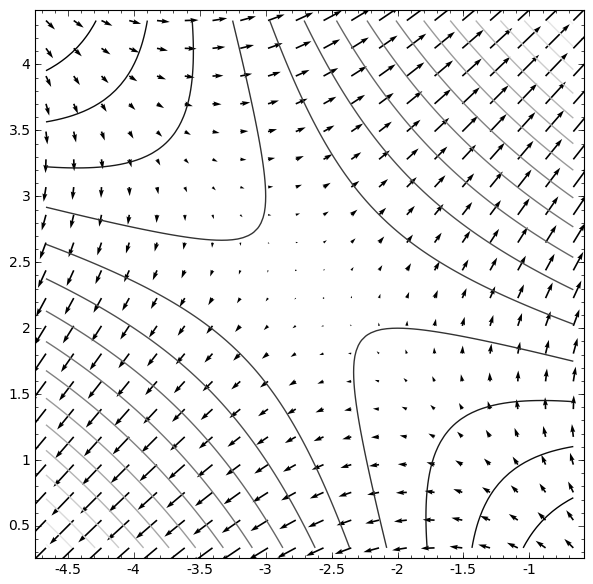
\includegraphics[width=\marginparwidth]{second-derivative-test.png}
}
 Consider the function $f(x,y)= x^2+4xy-4x+y^2+6y$. The derivative (gradient) is the vector field $Df(x,y) = (2x+4y-4,4x+2y+6)$. 
%See Figure \ref{second derivative graph} for a graph of several level curves, together with the gradient.
\begin{enumerate}
\item 
At what point(s) does $Df(x,y)=\vec 0$? These are the potential locations of maximums, minimums, or saddles.   
\item 
Compute the second derivative of $f$, which should give you a 2 by 2 symmetric matrix. This matrix is called the Hessian.
\item 
By looking at the plot to the right, are the eigenvalues of $D^2f(x,y)$ both positive, both negative, or do they differ in sign?  How can you tell? Then confirm you are correct by computing the eigenvalues and eigenvectors of $D^2f(x,y)$.  
\item 
Recall that the gradient points in the direction of greatest increase.  Using this information alone, does the function have a maximum, minimum, or saddle point.
\end{enumerate}

%\begin{figure}
% \begin{center}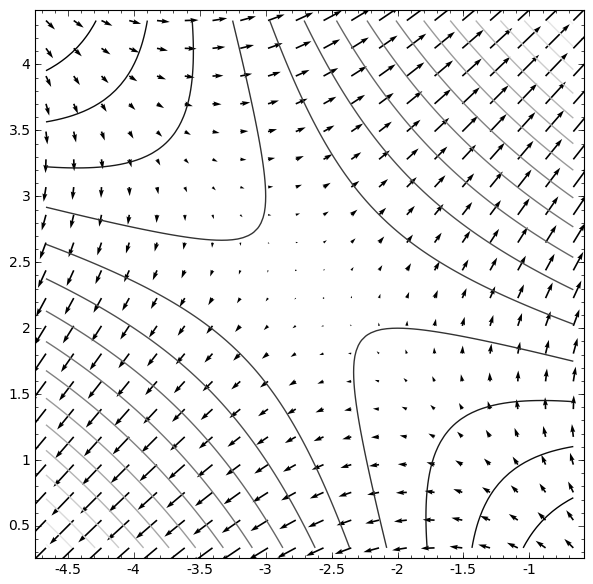
\includegraphics[width=\marginparwidth]{second-derivative-test.png}\end{center}
%\caption{A plot of several level curves of $f(x,y)=x^2+4xy-4x+y^2+6y$ and the gradient (the graph is not centered at the right spot, so ignore the axes). In one direction the gradient is pulling things towards the origin.  In another direction, the gradient is pushing things away from the origin. \label{second derivative graph}}
%\end{figure}
\end{problem}

We can summarize the results from the problem above into a theorem from multivariate calculus. 
\begin{theorem}
 Let $f(x,y)$ be a function that is twice continuously differentiable. Suppose that $Df(x,y)=(0,0)$ when $(x,y)=(a,b)$, so that $(a,b)$ is a critical point. To determine if the point $(a,b)$ corresponds to a maximum, minimum, or saddle point, we compute the eigenvalues of $D^2f(a,b)$ (the second derivative is called the Hessian).
\begin{itemize}
 \item If all eigenvalues are positive, then $f$ has a minimum at $(a,b)$. 
 \item If all eigenvalues are negative, then $f$ has a maximum at $(a,b)$. 
 \item If the eigenvalues differ in sign, then $f$ has a saddle at $(a,b)$. 
 \item If zero is an eigenvalue, then the second derivative test fails.
\end{itemize}
\end{theorem}



\mysubsection{\ideapro}

\begin{problem}
 Sally found the treasure in the corn field.  She's now looking for treasure in a swamp. There's a road through the swamp that runs parallel to the vector $\vec v=(3,4)$. Her current location is $(0,0)$ and the treasure (geocache) is located at the position $\vec b=(2,-4)$ (units are hundreds of yards). When Sally decides to leave the road, she'll have to wade through some swamp water. She would prefer to spend as little time in the swamp as possible. Her goal is to walk along the road until she reaches the point closest to the treasure, and then wade straight to the treasure.  This means she needs to find a scalar $c$ so that $c\vec v$ gets her as close to the treasure as possible. See the picture below. 
\begin{center}	
\begin{tikzpicture}[scale=1]
\draw[thin] (-3,-4) -- (3.3,4.4);
\draw [->,thick] (0,0) -- node [left=3pt]{$\vec v=(3,4)$}(3,4);
\draw [->,thick,red,dashed] (0,0) -- node [right=3pt]{$\vec b=(2,-4)$}(2,-4);
\draw [->,very thick,green] (0,0) -- node [left=3pt]{$c\vec v$}(-1.2,-1.6);
\draw [->,very thick,blue] (-1.2,-1.6) -- node [below=3pt]{$\vec n$}(2,-4);
\end{tikzpicture}
\quad 
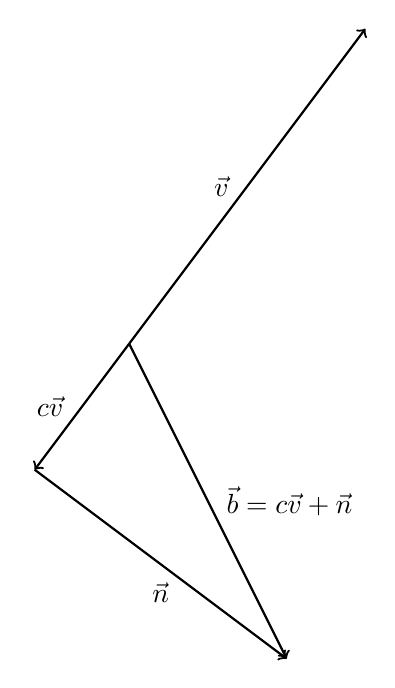
\begin{tikzpicture}[scale=1]
\draw [->,thick] (0,0) -- node [left=3pt]{$\vec v$}(3,4);
\draw [->,thick] (0,0) -- node [right=3pt]{$\vec b=c\vec v+\vec n$}(2,-4);
\draw [->,thick] (0,0) -- node [left=3pt]{$c\vec v$}(-1.2,-1.6);
\draw [->,thick] (-1.2,-1.6) -- node [below=3pt]{$\vec n$}(2,-4);
\end{tikzpicture}
\end{center}
The vector $\vec n$ represents the path she must take through the swamp. Her goal is to find a scalar $c$ so that $\vec b=c\vec v+\vec n$ and $\vec n$ is as short as possible. 
\begin{enumerate}
 \item What is the angle between $\vec v$ and $\vec n$? Why does $\vec v\cdot \vec n=0$?
 \item Sally knows that the treasure is at $\vec b = c\vec v+\vec n$.  Since $\vec v\cdot \vec n = 0$, she decides to dot both sides of this equation, on the left, by the vector $\vec v$ to get $\vec v\cdot \vec b = \vec v\cdot (c\vec v+\vec n)$. Show that in general $$c = \dfrac{\vec v\cdot \vec b}{\vec v\cdot \vec v} 
%= \dfrac{\vec v^T\vec b}{\vec v^T\vec v}.
$$ Then show that with Sally's specific road vector $\vec v$ and treasure vector $\vec b$, the constant $c$ is $c=-2/5$. 
% \item We know that $c\vec v$ is as close to $\vec b$ as you can get along the road. Since $\vec b = c\vec v+\vec n$ and we know $c\vec v$, solve for $\vec n$. Then find the distance Sally will have to travel in the swamp (what's the length of $\vec n$)? 
\end{enumerate}
 \end{problem}
 
The vector $c\vec v$ above is often called the orthogonal projection of $\vec b$ onto $\vec v$. The word orthogonal means that $\vec v\cdot \vec n=0$, i.e. that there is a 90 degree angle between $\vec v$ and $\vec n$. 
%The scalar $c$ is sometimes called a Fourier coefficient.    


\begin{problem}
 Now assume that Sally is an astronaut in space. She's moving through an asteroid field and knows there is safe passage if she follows the vector $\vec v = (1,-2,-3)$. She needs to get to the point $\vec b=(3,-6,-11)$. She already knows that if she follows $\vec v$ three times, she'll end up pretty close by arriving at $(3,-6,-12)$. However, she wants to follow $\vec v$ until she is as close to $\vec b$ as possible, as leaving the known safe path could be dangerous.  
\begin{enumerate}
 \item 
Determine the scalar $c$ so that $\vec v c$ is as close to $\vec b$ as possible. Your answer should be close to 3.  Use the formula from the previous problem.
  \item 
Let's swap to a different question. 
Suppose we would like to find an equation of a line $y=mx$ through the origin that passes through the three points  $(1,3)$, $(-2,-6)$, and $(-3,-11)$.
To pass through all three points we need to solve the system of equations $3=m(1)$, $-6=m(-2)$, and $-11=m(-3)$. 
Rewrite this system of equations as the vector equation (state $\vec v$ and $\vec b$) 
$$\vec v m = \vec b \quad\quad\quad\Rightarrow\quad\quad\quad \bvec{?\\?\\?}m = \bvec{?\\?\\?}.$$
Explain why there is no solution to this problem. 
  \item
What should we choose the slope $m$ to equal so that $\vec v m$ will be as close to $\vec b$ as possible? 
%[Hint: Multiply both sides on the left by the matrix $\vec v^T$.]
 \end{enumerate}
\end{problem}


\mysubsection{\ideacon}

Many problems in nature arise from conservation laws.  These laws generally focus on the principle that matter is neither created nor destroyed, rather it is just moved, changed, or something.  Any of the following could be viewed as a conservation law:
\begin{itemize}
 \item What comes in must come out.
 \item Voltage supplied equals voltage suppressed.
 \item Atoms before equal atoms after.
 \item The change in a quantity is how much it increases minus how much it decreases.
 \item Current in equals current out.
 \item The sum of the forces in every direction must match the total force.
 \item The force and moments must sum to zero when an object is at rest.
 \item This list could go on for a while.
\end{itemize}
Throughout this chapter, we'll see several different conservation laws.  You'll focus on understanding these conservation laws in your major classes. We'll see that almost every one of these problem can be written in the matrix form $A\vec x=\vec 0$. We'll see that $\lambda=0$ is an eigenvalue, which means that when we follow the eigenvector direction, the underlying vector field neither pushes outward nor inward. In this eigenvector direction, the system is conserving something.
\begin{definition}[Homogeneous System, Kernel]\label{homogeneous and kernel of a matrix}
Because we'll encounter problems of the form $A\vec x = \vec 0$ quite often, we make some definitions. 
\begin{itemize}
 \item We say that the linearly system $A\vec x=\vec b$ is homogeneous if $\vec b=\vec 0$. 
 \item The set of solutions to $A\vec x=\vec 0$ is called the kernel (or null space) of $A$.  
\end{itemize}
\end{definition}



Chemical reaction stoichiometry is the study of balancing chemical equations. A chemical reaction will often transform reactants into by-products. The by products are generally different compounds, together with either an increase or decrease in heat. One key rule in stoichiometry is that a chemical process neither creates nor destroys matter, rather it only changes the way the matter is organized. For simple reactions (with no radioactive decay), this conservation law forces the number of atoms entering a reaction to be the same as the number leaving. The next problem asks you to use this conservation law to create a balanced chemical reaction equation. 
\begin{problem}[Stoichiometry]
 The chemical compound hydrocarbon dodecane ($C_{12}H_{26}$) is used as a jet fuel surrogate (see Wikipedia for more info).  This compound reacts with oxygen $(O_2)$, and the chemical reaction produces carbon dioxide ($CO_2$), water ($H_2 O$), and heat.  Suppose we expose some dodecane to oxygen, and that a chemical reaction occurs in which the dodecane is completely converted to carbon dioxide and water.  
 Conservation requires that the number of atoms ($H$, $C$, and $O$) at the beginning of the chemical reaction must be the exact same as the number at the end. 
 We could write the chemical reaction in terms of molecules as
 $$x_1 C_{12}H_{26} +x_2 O_2 = x_3 CO_2+ x_4 H_2O\quad \text{or} \quad x_1 C_{12}H_{26} +x_2 O_2 - x_3 CO_2- x_4 H_2O=0, $$
 where $x_1$ molecules of dodecane and $x_2$ molecules of oxygen were converted to $x_3$ units of carbon dioxide and $x_4$ units of water.  
 If we look at each atom (carbon, hydrogen, and oxygen) individually, we obtain three equations to relate the variables $x_1, x_2, x_3, x_4$.  The carbon equation is simply
 $$x_1(12) + x_2(0) = x_3(1)+x_4(0) \quad \text{or}\quad x_1(12) + x_2(0) - x_3(1)-x_4(0)=0.$$  
 Your job follows:
\begin{enumerate}
 \item Write the other two conservation equations (for hydrogen and oxygen), and then organize your work into the matrix product $A\vec x = \vec 0$. This means you are working with a homogeneous system.
 \item Solve the corresponding system of equations by row reduction.  As there are only 3 equations with 4 unknowns, you should obtain infinitely many solutions. Write each variable in terms of the free variable.  You have found the kernel of the matrix $A$. 
 \item If about 10,000 molecules of water are present at the end of the reaction, about how many molecules of dodecane were burned? 
 \item 
\marginpar{If your answer on part 4 looks like your answer on the previous part, good. The point is that finding an eigenvector corresponding to $\lambda=0$ is the exact same as finding the kernel.}%
The matrix $A$ was not square.  We can make the system square by adding the trivial equation $0=0$, a row of zeros, to the bottom of the matrix. Let $B$ be this matrix. Why do we know $\lambda=0$ is an eigenvalue of this matrix?  Find an eigenvector corresponding to $\lambda=0$. 
\end{enumerate}
\end{problem}









\mysubsection{\idealin}


\begin{problem}\label{sally in city}
 After getting the treasure in the swamp, Sally moves on to find a treasure located in a small town. She has a map of the town that shows the city blocks.  However, when she looks at a satellite image of the city it's slightly different than her map. Here are the two maps (the city map is on the left, the satellite on the right).
 \begin{center}
 \begin{tabular}{cc}
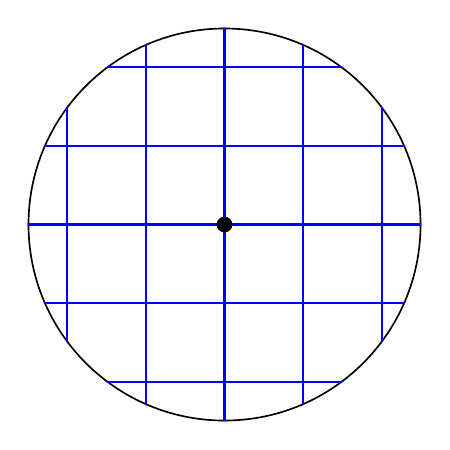
\begin{tikzpicture}
 \clip (0,0) circle (2.5cm);
 \draw[very thick] (0,0) circle (2.5cm);
 \foreach \x in {-3,-2,-1,0,1,2,3}
  \foreach \y in {-3,-2,-1,0,1,2,3}
   \draw[thick,blue] (\x,\y)--(\x+1,\y);
 \foreach \x in {-3,-2,-1,0,1,2,3}
  \foreach \y in {-3,-2,-1,0,1,2,3}
   \draw[thick,blue] (\x,\y)--(\x,\y+1);
 \fill (0,0) circle (.1cm);
 \end{tikzpicture}
&
 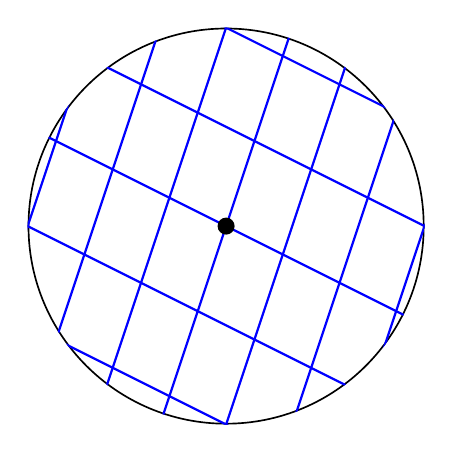
\begin{tikzpicture}[scale=.36]
 \clip (0,0) circle (7cm);
 \draw[very thick] (0,0) circle (7cm);
 \foreach \x in {-4,-3,-2,-1,0,1,2,3}
  \foreach \y in {-4,-3,-2,-1,0,1,2,3}
   \draw[thick,blue] (\x+2*\y,3*\x-\y)--(\x+1+2*\y,3*\x+3-\y);
 \foreach \x in {-4,-3,-2,-1,0,1,2,3}
  \foreach \y in {-4,-3,-2,-1,0,1,2,3}
   \draw[thick,blue] (\x+2*\y,3*\x-\y)--(\x+2*\y+2,3*\x-\y-1);  
 \fill (0,0) circle (.3cm);
%Eventually I would like to put the vectors in this problem. at nodes.  I don't know the syntax yet. 
%\draw node at (1,3) {$(0,0)$}
 \end{tikzpicture}
\\
City Map&Satellite View
 \end{tabular}
 \end{center}
 The city grid is not lined up with compass directions. When the city map tells her to go up one block, this really means her $(x,y)$ position should follow the vector $\vec v_1=(1,3)$. To go right 1 block, she follows the vector $\vec v_2=(2,-1)$. She has to learn to work with two different coordinate systems, namely the city coordinates (given in blocks) and the $(x,y)$ satellite coordinates (given in hundreds of yards). Assume that Sally is currently at the origin $(0,0)$. 
%She's currently standing at the point $A$ (which we'll consider the origin). Her GPS unit tells her that the treasure is located at the coordinates (). Our goal on this problem is to determine how she should follow the roads to get to the treasure.
\begin{enumerate}
 \item If Sally goes up 2 blocks, and right 3 blocks, what are here $(x,y)$ coordinates (in hundreds of yards)?
 \item If Sally moves up $c_1$ blocks and right $c_2$ blocks, then her $(x,y)$ coordinates are
$$\bvec{x\\y}=\bvec{1\\3}c_1+\bvec{2\\-1}c_2.$$ Rewrite this linear combination as a matrix product $A\bvec{c_1\\c_2}=\bvec{x\\y}$ (What is the matrix $A$?). You can check if you are correct by computing $A\bvec{1\\0}=\bvec{1\\3}$ and $A\bvec{0\\1}=\bvec{2\\-1}$. 
 \item If the treasure is located at the $(x,y)$ coordinates $(0,7)$, what directions would you give her in terms of blocks? If the treasure is located at $(1,-7.5)$, what directions would you give?
% \item What is the determinant of $A$? 
\end{enumerate}

\end{problem}


One way we can use a matrix is to think of the matrix as a map. When Sally was walking through the city in Problem \ref{sally in city}, she had a map of the city in her hands.  This map gave her the coordinates of locations in the city, but did so in a much simplified way. Going right on the map 1 block resulted in following the vector $(2,-1)$.  Going up 1 block resulted in following the vector $(1,3)$. It's much easier to give directions in terms of blocks.  

If Sally walks 2 blocks right, and 1 block up, then she arrives at $\bvec{2\\-1}(2)+\bvec{1\\3}(1) = \bvec{7\\1}$. In the city map, we base our all movement on the vectors $(1,0)$ and $(0,1)$. When looking at actual $(x,y)$ position, we base all our movements on the vectors $(2,-1)$ and $(1,3)$. We call each of these collections of independent vectors a basis.  We call $(c_1,c_2)=(2,1)$ the coordinates of the point $(x,y)=(7,1)$ relative to the basis $\{(2,-1),(1,3)\}$. 
We can describe any point $(x,y)$ using the simplified coordinates $(c_1,c_2)$ relative to this basis.


\begin{definition}[Basis and Coordinates Relative to a Basis]
 If the vectors $\vec v_1, \vec v_2,\ldots,\vec v_n$ are linearly independent, then we'll say these vectors form a basis.  
 We use the word ``basis'' because we can write (base) other vectors uniquely as a linear combination of these basis vectors.  You have been using the standard basis vectors $(1,0)$ and $(0,1)$ your entire life to talk about vectors in the plane. To plot the point $(2,3)$, we think ``right 2, up 3'' which is the same as the vector equation $(2,3)=2(1,0)+3(0,1)$. 

 Suppose $\mathscr{B}=\{\vec v_1, \vec v_2, \ldots, \vec v_n\}$ is a basis, and $\vec x$ is the linear combination
 $$\vec x = \vec v_1c_1+\vec v_2c_2+\cdots +\vec v_n c_n.$$
 Then we call $c_1, c_2, \ldots,c_n$ the coordinates of $\vec x$ relative to the basis $\mathscr{B}$. 
 
 In terms of matrices, when the columns of $A$ are linearly independent and $A\vec c=\vec x$, we say that $\vec c$ is the  coordinates of $\vec x$ relative to the columns of $A$. 
\end{definition}

A matrix $A$ takes each coordinate $(c_1,c_2)$ and transforms it to the point $\bvec{x\\y}=A\bvec{c_1\\c_2}$. You'll see in the next problem that lines get transformed to lines. For this reason, and others we'll soon see,  we call this coordinate transformation map a linear transformation. 

\begin{problem}\label{candice's treasure}
 Consider the matrices $A=\bvec{\nvec{1\\2}&\nvec{-1\\4}}$ and $B=\bvec{\nvec{1\\2}&\nvec{3\\-2}}$.  
 \begin{enumerate}
  \item 
  Consider  
  $\bvec{\nvec{1\\2}&\nvec{-1\\4}&\nvec{-1\\10}&\nvec{3\\0}&\nvec{1\\2}&\nvec{1\\0}}
  \xrightarrow{rref}
  \bvec{\nvec{1\\0}&\nvec{0\\1}&\nvec{1\\2}&\nvec{2\\-1}&\nvec{1\\0}&\nvec{2/3\\-1/3}}
  $.
  
  If we want to write $(x,y)=(-1,10)$ as a linear combination of the columns of $A$, what scalars (coordinates) $c_1$ and $c_2$ give $\pvec{1\\2}c_1+\pvec{-1\\4}c_1=\pvec{-1\\10}$?
  
  What are the coordinates of $(x,y)=(3,0)$ relative to the columns of $A$?  

  What are the the coordinates of $(1,0)$ relative to the basis $\{(1,2), (-1,4)\}$?
  \item
 Alice decides to walk around using coordinates relative to the columns of $A$.  She starts at $(0,0)$, and then walks to the $(c_1,c_2)$ coordinates $(1,0)$, then $(1,2)$, then $(0,1)$, and then back to $(0,0)$. Her path in the $(x,y)$ plane is shown below on the right.  
 \begin{center}
\newcommand{\mux}{1}
\newcommand{\muy}{2}
\newcommand{\mvx}{-1}
\newcommand{\mvy}{4}
\begin{tikzpicture}
\node (A) at (0,0) {\begin{tikzpicture}
  axis
  \draw (-1,0) -- coordinate (x axis mid) (2,0);
  \draw (0,-1) -- coordinate (y axis mid) (0,3);
  ticks
  \foreach \x in {-1,...,2}
   \draw (\x,1pt) -- (\x,-3pt)
    node[anchor=north] {};
  \foreach \y in {-1,...,3}
   \draw (1pt,\y) -- (-3pt,\y) 
    node[anchor=east] {}; 
  \fill[opacity=.2] (0,0) -- (1,0) -- (1,2) -- (0,1) -- (0,0);
  \draw[red,->,very thick] (0,0)--(1,0);
  \draw[blue,->,very thick] (0,0)--(0,1);
  \node at (.5,-1.5) {Coordinates $(c_1,c_2)$};
\end{tikzpicture}};
\node[right=of A ] (B) {\begin{tikzpicture}[scale=.5]
  axis
  \draw (-2,0) -- coordinate (x axis mid) (2,0);
  \draw (0,-1) -- coordinate (y axis mid) (0,10);
  ticks
  \foreach \x in {-2,...,2}
   \draw (\x,1pt) -- (\x,-3pt)
    node[anchor=north] {};
  \foreach \y in {-1,...,10}
   \draw (1pt,\y) -- (-3pt,\y) 
    node[anchor=east] {}; 
  \fill[opacity=.2] (0,0) -- (\mux,\muy) -- (\mux+2*\mvx,\muy+2*\mvy) -- (\mvx,\mvy) -- (0,0);
  \draw[red,->,very thick] (0,0)--(\mux,\muy);
  \draw[blue,->,very thick] (0,0)--(\mvx,\mvy);
  \node at (-2,-1.5) {Position $(x,y)$};
 \end{tikzpicture}};
 \draw[->] (A.east) -- node[above=3pt]{\footnotesize $A\bvec{c_1\\c_2} = \bvec{x\\y}$} (B.west);
\end{tikzpicture}
\end{center}
Bob decides to follow the same coordinate path, but he's using coordinates relative to the columns of $B$.  Draw Bob's path in the $(x,y)$ plane.  Remember that since we know coordinates $(c_1,c_2)$, we can get the $(x,y)$ position from $B\bvec{c_1\\c_2}=\bvec{x\\y}$. 

 
 %(How can you tell that Bob got his map by taking a picture of someone else map in a mirror?)
%I chose a bad matrix, because you loose the entire point to this problem.  It looks bad when you graph it, because something lines up perfectly. 
  \item 
 Candice is staring at a treasure map.  She doesn't have a matrix $C$ to help her translate from the treasure map to actual $(x,y)$ points. However, she does have a few bits of information. There are two trees on her map with coordinates $(c_1,c_2)$ at $(2,1)$ and $(-4,-3)$. The actual $(x,y)$ location of these trees is $(-4,5)$ and $(7,-10)$  This means if Candice knew $C$, then she could compute $C\bvec{\nvec{2\\1}}=\bvec{\nvec{-4\\5}}$ and $C\bvec{\nvec{-4\\-3}}=\bvec{\nvec{7\\-10}}$.  Combining these two products together into one matrix means $$C\bvec{\nvec{2\\1}&\nvec{-4\\-3}}=\bvec{\nvec{-4\\5}&\nvec{7\\-10}}.$$  Use this to find $C$.  [Hint: Try using an inverse matrix.]
 \item The treasure on Candice's map has the map coordinates $(-1,5)$.  Give Candice the $(x,y)$ location of the treasure.   
 \end{enumerate}

\end{problem}







%7










%7 - Adjoint Problem


\begin{problem}
Consider the matrix
$A=\begin{bmatrix}
2&1&-1\\1&2&0\\0&4&3 
\end{bmatrix}.$
\begin{enumerate}
 \item 
 Compute the determinant of $A$. 
 \item 
\marginpar{If you forgot what a cofactor is, you'll want to review the definition.  See Definition \ref{general determinants} on page \pageref{general determinants}. }%
Now create a matrix $B$ so that the $ij$th entry of $B$ is the cofactor $C_{ij}$ (remove row $i$ and column $j$, compute the determinant, and then times by an appropriate sign).  
This will require that you compute nine 2 by 2 determinants.  
 \item 
Compute the inverse of $A$ with software. 
 \item 
Make a conjecture about the connection between the determinant of $A$, this matrix of cofactors $B$, and the inverse of $A$.  
\end{enumerate}
%We'll verify your conjecture is true on a 4 by 4 matrix in class. 
\end{problem}


In your work above, you should have noticed that you had to interchange the rows and columns of $B$ to make your conjecture.  This process of interchanging rows and columns, called transposing a matrix, will show up in so many of our applications that we make a definition.

\begin{definition}[The Transpose $A^T$. Symmetric Matrix]
 If $A$ is an $m$ by $n$ matrix, then the transpose of $A$ is the $n$ by $m$ matrix formed by interchanging the rows and columns.  Row 1 is now column 1. Row 2 is now column 2.  Just think of each row as a vector, and then place those vectors in the columns of a new matrix.  We use the symbol $A^T$ to stand for the transpose of a matrix.

We'll often encounter square matrices where the transpose of the matrix is the matrix itself.  If $A=A^T$ then we say the matrix is symmetric. When a vector field has a potential, its derivative satisfies this property. 
\end{definition}









%8
\begin{problem}
\marginpar{
For the matrix $A=\bvec{2&1\\0&3}$, you should see the two pictures below.

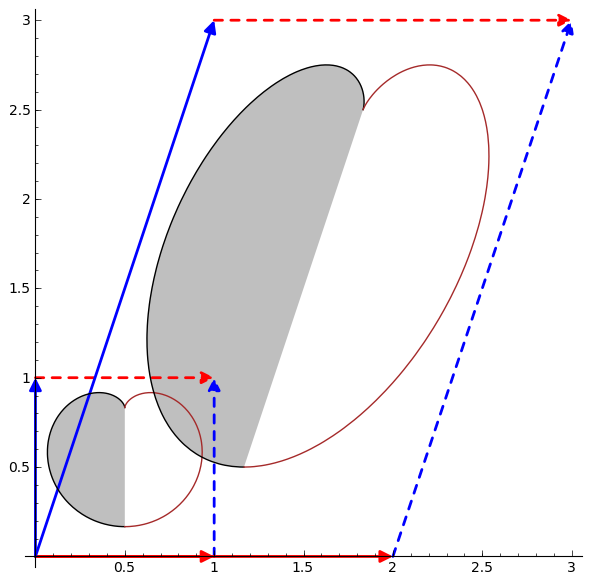
\includegraphics[width=\marginparwidth]{lineartransformation1.png}

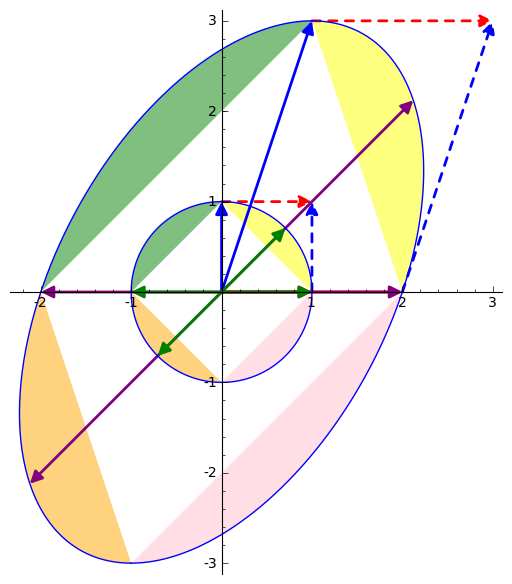
\includegraphics[width=\marginparwidth]{lineartransformation2.png}
}%
 On this problem, you will explore graphs of several linear transformations. Your job is to look for patterns and explanations.  Please head to the following webpage:
\begin{itemize}
 \item \href{\urllineartransformationsinplane}{\urllineartransformationsinplane}
\end{itemize}
You may find this problem easiest if you create your own account at sagemath.org, and then copy the code from the URL above to your own notebook. Then you can put 10+ linear transformation graphs in the same document so you can compare them all side by side. 

Here's your job. In the software link above, change the matrix $A$ to be several different matrices. Look for an answer to each question below.
\begin{itemize}
 \item What does the determinant tell you about the map? Can you see the determinant in the pictures?
 \item If the determinant is zero, what does that mean about your map?
 \item What do the eigenvalues tell you about your map? This is perhaps easiest to tell with the circle map.
 \item Is there a connection between the eigenvalues and the determinant?
 \item What do the eigenvectors tell you?
 \item Does anything special happen if the matrix is symmetric?
\end{itemize}
To be prepared for class, write answers to at least 4 of these questions using complete sentences.
There are many great answers to the questions above. 

Here are some matrices that might be useful to look at. Please type each of these in.  As you discover patterns, test them against these matrices. 
$$
\bvec{2&1\\0&3},
\bvec{-2&1\\0&3},
\bvec{-2&1\\0&-3},
\bvec{0&4\\3&1},
\bvec{2&1\\1&2},
\bvec{1&2\\2&4},
\bvec{0&-1\\1&0},
\bvec{-1&2\\2&1},
$$
$$\bvec{\cos(pi/3)&-\sin(pi/3)\\ \sin(pi/3)&\cos(pi/3)},
\bvec{3\cos(pi/6)&-5\sin(pi/6)\\ 3\sin(pi/6)&5\cos(pi/6)}.
$$
\end{problem}
%end 8

















%9
\mysubsection{\ideanon}
\begin{problem}
\marginpar{
Here's a plot of several level curves of $f(x,y)=x^3-3x^2-y^2+2y$ and the gradient. There are two critical points.  

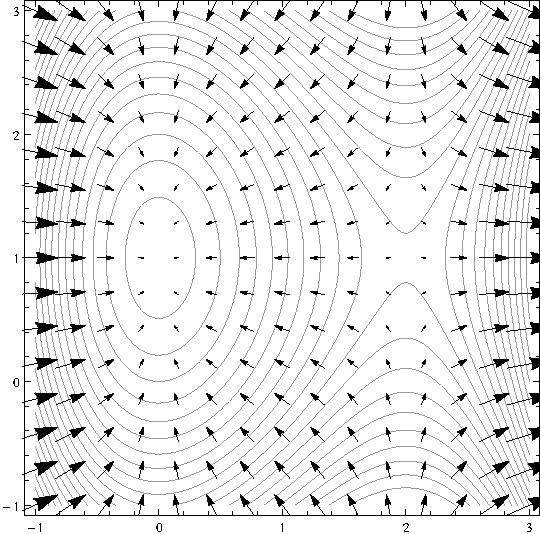
\includegraphics[width=\marginparwidth]{second-derivative-test2}
}%
 Consider the function $f(x,y) = x^3 - 3x ^2 - y^2 + 2y$
\begin{enumerate}
\item 
At what point(s) does $Df(x,y)=\vec 0$? You should obtain two points. These are the potential locations of maximums, minimums, or saddles.   
 \item 
Compute the second derivative of $f$, which is a 2 by 2 symmetric matrix. 
 \item 
Pick one of the critical points. Use the vector field plot to the right to decide if the eigenvalues of $D^2f(x,y)$ are both positive, both negative, or differ in sign at that critical point. Then state if the function has a maximum, minimum, or saddle at that point.  Then repeat with the other critical point. 
 \item 
Now compute the eigenvalues of the Hessian at each critical value. You'll need to find the eigenvalues of two different matrices.  This should confirm your answer to part 3. (The matrix is diagonal, so computing eigenvalues should be quick.)  
Don't forget that you are finding eigenvalues of $D^2f(a,b)$, not $D^2f(x,y)$. 
\end{enumerate}
\end{problem}


The following example adds a little more information to this discussion. I've included it to give you one additional piece of information, namely how the eigenvalues and eigenvectors connect to the concavity of the function. 

\begin{example}
For the function {$f(x,y)=x^2+xy+y^2$}, the gradient is $Df = \begin{bmatrix}2x+y&x+2y \end{bmatrix}$, which is zero only at $x=0,y=0$ (solve the system of equations $2x+y=0,x+2y=0$). The Hessian is $D^2f = \begin{bmatrix}2&1 \\1&2\end{bmatrix}$. The eigenvalues are found by solving $0=\det \begin{bmatrix}2-\lambda &1 \\1&2-\lambda \end{bmatrix} = (2-\lambda)^2-1 = 4-4\lambda+\lambda^2 -1 = (\lambda-3)(\lambda-1)$, so $\lambda = 3,1$ are the eigenvalues.  Since both eigenvalues are positive, the gradient pushes things away from the origin in all direction, which means in every direction you move from the critical point, you'll increase in height.  There is a minimum at $(0,0)$.  

The eigenvectors of the Hessian help us understand more about the graph of the function.  An eigenvector corresponding to 3 is $(1,1)$, and corresponding to 1 is $(-1,1)$. These vectors are drawn in figure \ref{2ndder}, together with two parabolas whose 2nd derivatives are precisely 3 and 1.  The parabola which opens upwards the most quickly has a 2nd derivative of 3.  The other parabola has a second derivative of 1. In every other direction, the 2nd derivative would be between 1 and 3.
\end{example}

%\marginpar{{
\begin{figure}[ht
]\begin{center}
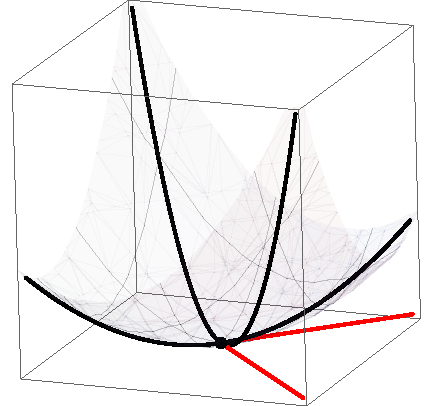
\includegraphics[width=2in]{support/2nddertest1}
\hspace{.5in}
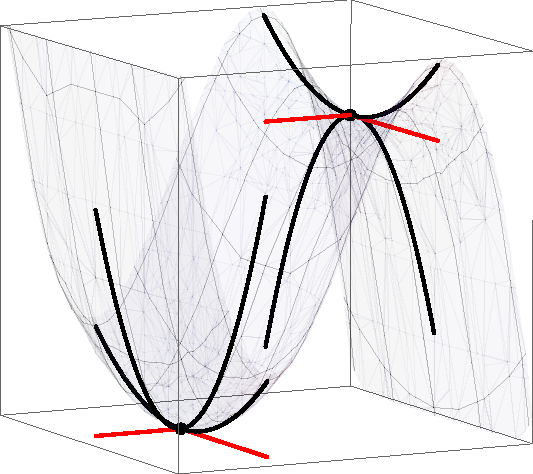
\includegraphics[width=2in]{support/2nddertest2}
\end{center}
\caption{The eigenvectors of the second derivative tell you the directions in which the 2nd derivative is largest and smallest. At each critical point, two eigenvectors are drawn as well as a parabola whose second derivative (the eigenvalue) matches the second derivative of the surface in the corresponding eigenvector direction.}
\label{2ndder}
\end{figure}
%}}
%end 9
















%10
\mysubsection{\ideapro}
\begin{problem}
Jimmy is using a rocket suit to travel out in space. His rocket suit had 4 good boosters that allowed travel in any direction, with a backup booster in case one got damaged.  However, some tiny meteorites happened to pass by and take out two of his boosters, as well as his radio to call for help.  He's now only able to move in the directions $\vec v_1=(1,1,1)$ and $\vec v_2=(-1,1,2)$.  His space ship is sitting at $\vec b=(-1,4,7)$.
\begin{enumerate}
 \item 
 Show that Jimmy cannot arrive at his ship using his two working boosters.  In other words, show that we cannot write $\vec b$ as a linear combination of $\vec v_1$ and $\vec v_2$? Set up an appropriate matrix equation, row reduce the equation, and use your row reduction to give an answer. 
 \item 
 Jimmy has a one shot back up gun.  This gun will propel him towards the ship if he points the gun directly away from the ship and fires.  
 It's easy to miss aim, so he would like to get as close to the ship as possible before he fires the gun. 
 He needs to find $c_1$ and $c_2$ so that $\vec w = \vec v_1 c_1+\vec v_2 c_2$ gets him as close to the ship as possible. The picture below illustrates the general idea. The vectors $\vec v_1$ and $\vec v_2$ give Jimmy a plane of possible movements. 
\begin{center}	
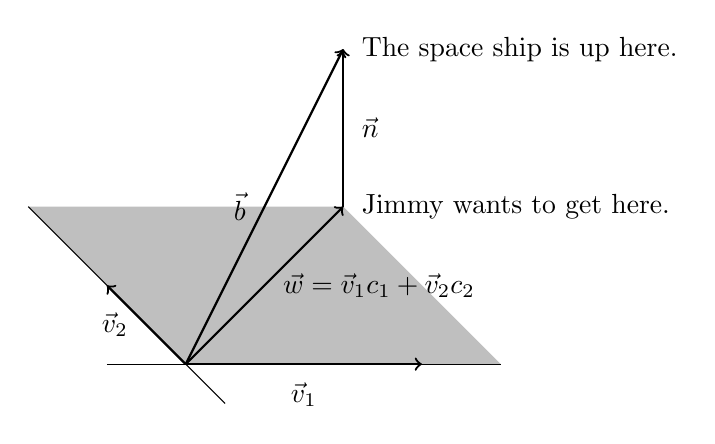
\begin{tikzpicture}[scale=1]
\fill[lightgray] (0,0) -- (-2,2) -- (2,2) -- (4,0) -- (0,0);
\draw[thin] (-1,0) -- (4,0);
\draw[thin] (.5,-.5) -- (-2,2);
\draw [->,thick] (0,0) -- node [below=3pt]{$\vec v_1$}(3,0);
\draw [->,thick] (0,0) -- node [left=3pt]{$\vec v_2$}(-1,1);
\draw [->,thick] (0,0) -- node [left=3pt]{$\vec b$}(2,4) node[right=3pt]{The space ship is up here.};
\draw [->,thick] (0,0) -- node [right=3pt]{$\vec w = \vec v_1 c_1+\vec v_2 c_2$}(2,2) node[right=3pt]{Jimmy wants to get here.};
\draw [->,thick] (2,2) -- node [right=3pt]{$\vec n$}(2,4);

%\draw [->,thick] (-1.2,-1.6) -- node [below=3pt]{$\vec n$}(2,-4);
\end{tikzpicture}
\end{center}
 When Jimmy has arrived at the closest spot to the ship, he'll have the smallest $\vec n$ so that 
$$\vec v_1 c_1+\vec v_2 c_2+\vec n=\vec b\quad\quad\text{ or }
\quad \quad 
\pvec{1\\1\\1} c_1+\pvec{-1\\1\\2} c_2+\vec n=\pvec{-1\\4\\7}.$$ Why must $\vec v_1^T\vec n=0$ and $\vec v_2^T\vec n=0$?  
 \item 
 Since there are two unknown constants $c_1$ and $c_2$, we need two equations.  Multiply both sides of the above equation on the left by $\vec v_1^T=\bvec{1&1&1}$. Why does $\vec n$ vanish from the equation? This gets us one equation.
 \item 
 To get a second equation, we multiply both sides by $\vec v_2^T=\bvec{-1&1&2}$. We now have two equations with two unknowns $c_1$ and $c_2$. Solve and show that $c_1 = 11/7$ and $c_2=37/14$.
% \item 
% Let $A =\bvec{\vec v_1&\vec v_2} = \bvec{1&-1\\1&2\\1&2}$. What does $A^TA$ and $A^T$ 
% You can organize all your work above into a single equation. Show that solving $A^TA\vec x = A^T\vec b$ for $\vec x$. 
\end{enumerate}

\end{problem}

The problem above asked you to find the point in a plane that was closest to a point not on the plane.  This is called the orthogonal projection of $\vec b$ onto the plane formed by the vectors $\vec v_1$ and $\vec v_2$.  If we let $A=\bvec{\vec v_1&\vec v_2}$, then the projection of $\vec b$ onto this plane is $w=\vec v_1c_2+\vec v_2c_2=A\bvec{c_1\\c_2}$. Our goal is to find $\bvec{c_1\\c_2}$ such that $\vec n=\vec b-A\bvec{c_1\\c_2}$ is as short as possible. The next problem shows that you can accomplish this by solving $A^TA\vec x=A^T\vec b$ for $\vec x$. We just take the problem $A\vec x=\vec b$ which has no solution, multiply both sides by $A^T$, and then solve.  
%end 10




 
 
 



%11
\begin{problem}
 Suppose we would like to find an equation of a line $y=a_0+a_1x$ that passes through the three points 
 $(-1,-1)$, $(1,4)$ and $(2,7)$. If such a line does not exist, we'd like to find a line that passes close to these three points. 
 \begin{enumerate}
  \item The three points give us three equations that involve the unknown constants $a_0$ and $a_1$. Show that we can write these equations in the matrix form $A\vec x = \vec b$ and vector form $\vec v_1a_0+\vec v_2a_1 = \vec b$ 
  $$\bvec{1&-1\\1&1\\1&2}\bvec{a_0\\a_1}=\bvec{-1\\4\\7}\quad\quad\text{or}\quad\quad \bvec{1\\1\\1}a_0+\bvec{-1\\1\\2}a_1=\bvec{-1\\4\\7}.$$
  Then show that there is no solution to this problem.
  \item We now know that no linear combination of $\vec v_1=(1,1,1)$ and $\vec v_2 =(-1,1,2)$ will give us the vector $\vec b=(-1,4,7)$.  We would like to find scalars $a_0$ and $a_1$ so that $\vec v_1a_1+\vec v_2a_1$ is as close to $\vec b$ as possible. This is the exact same question as the previous problem (where Jimmy could not get to his space ship). 
  Multiply both sides of the inconsistent equation $A\vec x = \vec b$ on the left by $\bvec{1\\1\\1}^T = \bvec{1&1&1}$, and then multiply both sides by  $\bvec{-1\\1\\2}^T = \bvec{-1&1&2}$. This should get you two different equations that involve $c_1$ and $c_2$. 
  \item Compute $A^TA = \bvec{1&1&1\\-1&1&2}\bvec{1&-1\\1&1\\1&2}$ and $A^T\vec b=\bvec{1&1&1\\-1&1&2}\bvec{-1\\4\\7}$.  You should see that both of your equations above are in the matrix equation  
  $$A^TA\vec x=A^T\vec b \quad \Rightarrow \quad \bvec{1&1&1\\-1&1&2}\bvec{1&-1\\1&1\\1&2}\bvec{a_0\\a_1}=\bvec{1&1&1\\-1&1&2}\bvec{-1\\4\\7}.$$ 
Make sure you simplify the matrix products $A^TA$ and $A^T\vec b$, as this should become a system of 2 equations and 2 unknowns. 
  \item Now solve $A^TA\vec x = A^T\vec b$ for $\vec x = \bvec{a_0\\a_1}$. Use your answer to state the line  $y=a_0 +a_1x$ that passes nearest these three points. 
 \end{enumerate}
\end{problem}
 
 The transpose of a matrix plays a crucial role in finding projections. When the problem $A\vec x =\vec b$ has no solution, it is impossible to write $\vec b$ as a linear combination of the columns of $A$.  If we multiply both sides on the left by $A^T$, then we have an equation that we can solve to obtain the coefficients $\vec x$ so that $A\vec x$ is as close to $\vec b$ as possible. This is the key idea to regression. 
%end 11







 
 
 


\mysubsection{\ideacon}
% 12
When we perform a partial fraction decomposition, Our goal is to rewrite a complicated fraction as the sum of simpler fractions.  We are not changing the quantity that the fraction represents, rather we are just changing how we express the fractions.  This is a conservations law, as the fractional quantity is conserved.  Can we answer this problem by looking for the kernel of some matrix, or an eigenvector corresponding to $\lambda=0$?

\begin{problem}\label{partial fraction general solution}
Consider the partial fraction decomposition 
$$
\frac{8s+7}{(s-2)(s+3)} = \frac{A}{s-2}+\frac{B}{s+3}
$$
which we  can rewrite in the form
$$8s+7 = A(s+3)+B(s-2).$$
Let's compare several different ways of solving this problem.
\begin{enumerate}
 \item Complete this partial fraction decomposition. Use any method you like. 
 \item Now let's solve 
$$
\frac{cs+d}{(s-2)(s+3)} = \frac{A}{s-2}+\frac{B}{s+3}
$$
Rather than thinking of $c$ and $d$ as known constants, let's make them variables in our linear system of equations.  
Our goal is to solve 
$$
(A+B-c)s+(3A-2B-d)=0
$$   
which we can rewrite in the matrix form 
\marginpar{Why did I save the last two columns for $c$ and $d$?}%
$$\bvec{
1 & 1 & -1 & 0 \\
3 & -2 & 0 & -1
}\bvec{A\\B\\c\\d}=\bvec{0\\0}.$$
This is a matrix equation of the form $A\vec x=\vec 0$, so the solutions are the kernel of $A$. Solve this matrix equation (find the kernel of $A$) and write your answer in terms of the free variables. Please use software to row reduce, and just share the key parts of your work (as shown below).
$$\bvec{[cccc|c]*&*&*&*&*\\ *&*&*&*&*}\xrightarrow{\text{rref}}\bvec{[cccc|c]1&0&*&*&*\\ 0&1& *&*&*}\Rightarrow \pvec{A\\B\\c\\d}=\bvec{*\\ *\\ *\\ * }c+\bvec{*\\ *\\ *\\ * }d.$$

% \item 
% We can rewrite the two equations $c=c$ and $d=d$ as the equations $0=0$ and $0=0$. Adding two rows of zeros to our matrix equation yields
% $$\bvec{
% 1 & 1 & -1& 0 \\
% 3 &-2 & 0 & -1\\
% 0 & 0 & 0 & 0\\
% 0 & 0 & 0 & 0
% }\bvec{A\\B\\c\\d}=\bvec{0\\0\\0\\0}.$$
% Can you explain, from the definition of eigenvalues, why $\lambda =0$ is an eigenvalue of this matrix? Then find all eigenvectors of this matrix corresponding to $\lambda=0$.

\item 
Change the 2 by 4 matrix above to solve the partial fraction decomposition
$$
\frac{cs+d}{(s-p)(s-q)} = \frac{A}{s-p}+\frac{B}{s-q}.
$$
Then use software to solve, giving $A$ and $B$ in terms of $c,d,p,q$. %Under what conditions will your solution fail?
\end{enumerate}
\end{problem}
%end 12









% 13
%Traffic flow application
\begin{problem}[Traffic Flow]
Consider the following traffic flow grid.
\begin{center}
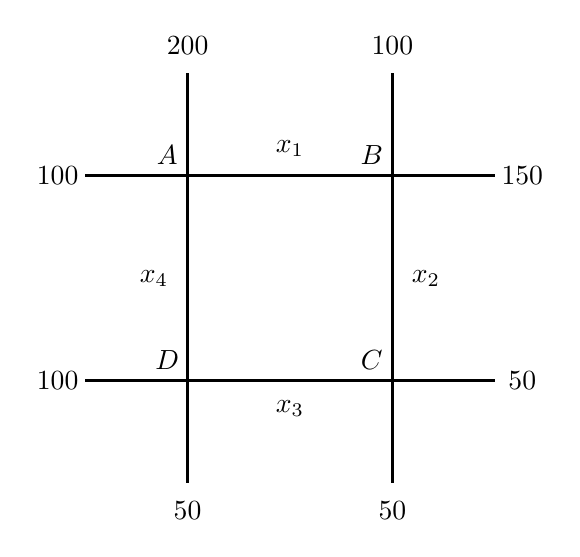
\begin{tikzpicture}[scale=1.3]
\begin{scope}[very thick, every node/.style={sloped,allow upside down}]
%\draw[step=1cm,gray,very thin] (-2,-2) grid (2,2);
\draw (-2,1)-- node(A) {\midarrow} (-1,1); 
\draw (-1,2)-- node(B) {\midarrow} (-1,1);  
\draw (1,1)-- node(C) {\midarrow} (1,2) ;  
\draw (1,1)-- node(D) {\midarrow} (2,1) ;  
\draw (2,-1) -- node(E) {\midarrow} (1,-1) ;  
\draw (1,-2) -- node(F) {\midarrow} (1,-1) ;  
\draw (-1,-1) -- node(G) {\midarrow} (-1,-2) ;  
\draw (-1,-1) -- node(H) {\midarrow} (-2,-1) ;  
\draw (-1,1) -- node(I) {\midarrow} (1,1) ;  
\draw (-1,1) -- node(J) {\midarrow} (-1,-1) ;  
\draw (1,-1) -- node(K) {\midarrow} (1,1) ;  
\draw (1,-1) -- node(L) {\midarrow} (-1,-1) ;  
\end{scope}
\draw (-1,1)  ++(-.2,.2) node {$A$}; 
\draw (1,1)  ++(-.2,.2) node {$B$}; 
\draw (1,-1)  ++(-.2,.2) node {$C$}; 
\draw (-1,-1)  ++(-.2,.2) node {$D$}; 
\node[left of=A] {100};
\node[above of=B] {200};
\node[above of=C] {100};
\node[right of=D] {150};
\node[right of=E] {50};
\node[below of=F] {50};
\node[below of=G] {50};
\node[left of=H] {100};
\node[label=above:$x_1$] at (I){};
\node[label=right:$x_2$] at (K){};
\node[label=below:$x_3$] at (L){};
\node[label=left:$x_4$] at (J){};
\end{tikzpicture}
\end{center}
The numbers on the edges represent the number of vehicles that either enter or leave the system each hour.  The variables $x_1$, $x_2$, $x_3$, and $x_4$ represent the number of cars on each road. Assume that all streets are one-way streets where the arrows give the direction of traffic flow.
\begin{enumerate}
 \item How do you know there are 400 total cars entering this network of roads each hour? Are all these cars leaving? This is a conservation problem?
 \item The number of cars entering an intersection must match the number of cars leaving an intersection.  We can use this to build a system of equations for the traffic flows $x_1, x_2,x_3, x_4$.  Every hour at node $A$ there are 300 cars entering the intersection and $x_1+x_4$ cars leaving the intersection. This gives us an equation $x_1+x_4=300$. Continue in this fashion to obtain an equation at each intersection point. You should have a system of 4 equations with 4 unknowns.
 \item 
Write your system of equations in the matrix form $A\vec x = \vec b$. What is $A$, what is $\vec x$, and what is $\vec b$? Is this system homogeneous or non homogeneous? 
 \item Solve your system of equations.  When you are presenting this kind of information in class, you should use the pattern $B\xrightarrow{\text{rref}}R\Rightarrow\vec x = ...$, so show us the augmented matrix $B$, show us its rref $R$, and then state the solution $\vec x$ as a linear combination of vectors, namely
$$
\bvec{[cccc|c]*&*&*&*&*\\ *&*&*&*&*\\ *&*&*&*&*\\ *&*&*&*&*}
\xrightarrow{\text{rref}}\bvec{[cccc|c]1&0&0&*&*\\ 0&1&0&*&*\\ 0&0&1&*&*\\ 0&0&0&0&0}\Rightarrow \pvec{x_1\\x_2\\x_3\\x_4}=\bvec{*\\ *\\ *\\ * }x_4+\bvec{*\\ *\\ *\\ * }.$$

 \item (Challenge - we'll answer in class if you're unable) What's the minimum number and maximum number of cars that can be on the road $AD$ each hour? Explain.
\end{enumerate}
\end{problem}

Whenever I see a problem that involves a conservation law, I think two things. For one, there is probably a homogeneous system $A\vec x = \vec 0$ somewhere in the background whose kernel is the solution. Two, if I make sure $A$ is a square matrix (possibly adding rows of zeros), then I can rephrase ``find the kernel'' as ``find the eigenvectors corresponding to zero.'' To accomplish finding this matrix $A$, we'll often have to think of given constants as variables.  Let's do this with the previous problem. 

\begin{problem}
Use the same setting as the previous traffic flow problem, however, let's change the given values to be variables.  Starting in the upper left corner and moving clockwise, replace the numbers 100, 200, 100, 150, etc., with the variables $a$, $b$, $c$, $d$, $e$, $f$, $g$, $h$. We now have 12 unknowns, namely $x_1$, ..., $x_4$, $a$, $b$, ..., $h$. 
\begin{enumerate}
 \item  At node $A$, our equation is now $x_1+x_4-a-b=0$. Write the other 3 equations and express the homogeneous system in the form $A\vec x = \vec 0$ where $A$ is a 4 by 12 matrix.  State the matrix $A$.
 \item Find the kernel of $A$, and write your solution as a linear combination of vectors where the scalars are the free variables (use the $B\xrightarrow{\text{rref}}R\Rightarrow\vec x = ...$ pattern). Your solution should look like 
$$
\bvec{x_1\\ x_2 \\ x_3\\ x_4\\a\\b\\c\\d\\e\\f\\g\\h}=
\bvec{*\\ *\\ *\\ *\\ *\\ *\\ *\\ *\\ *\\ *\\ *\\ *}x_4+
\bvec{*\\ *\\ *\\ *\\ *\\ *\\ *\\ *\\ *\\ *\\ *\\ *}b+
\bvec{*\\ *\\ *\\ *\\ *\\ *\\ *\\ *\\ *\\ *\\ *\\ *}c+
\bvec{*\\ *\\ *\\ *\\ *\\ *\\ *\\ *\\ *\\ *\\ *\\ *}d+
\bvec{*\\ *\\ *\\ *\\ *\\ *\\ *\\ *\\ *\\ *\\ *\\ *}e+
\bvec{*\\ *\\ *\\ *\\ *\\ *\\ *\\ *\\ *\\ *\\ *\\ *}f+
\bvec{*\\ *\\ *\\ *\\ *\\ *\\ *\\ *\\ *\\ *\\ *\\ *}g+
\bvec{*\\ *\\ *\\ *\\ *\\ *\\ *\\ *\\ *\\ *\\ *\\ *}h.
$$ 
%\item Rewrite your solution, ignoring the rows corresponding to the free variables. Your answer should look like
%$$
%\bvec{x_1\\ x_2 \\ x_3\\a}=
%\bvec{*\\ *\\ *\\ *}x_4+
%\bvec{*\\ *\\ *\\ *}b+
%\bvec{*\\ *\\ *\\ *}c+
%\bvec{*\\ *\\ *\\ *}d+
%\bvec{*\\ *\\ *\\ *}e+
%\bvec{*\\ *\\ *\\ *}f+
%\bvec{*\\ *\\ *\\ *}g+
%\bvec{*\\ *\\ *\\ *}h.
%$$ 
\item 
The 4th row of your rref is not zero (which is why $a$ is not a free variable).  
Write the equation given by this 4th row.  Can you interpret this 4th equation as a conservation law?
\end{enumerate}
\end{problem}
%end 13









\mysubsection{\idealin}

Have you noticed in every matrix problem we can always write the solution as a linear combination of vectors? 
When the system is homogeneous, the solution to $A\vec x = \vec 0$ (the kernel) is always all linear combinations of a few vectors. We take a vector times a free variable, plus a vector times a free variables, etc. The solution is the set of all linear combinations of a few vectors. It would be nice to say ``all linear combinations of'' in an efficient way. We'll use the word span to talk about forming all linear combinations, the word vector space to talk about the vectors in the span, and then dimension to talk about the geometric size of the span (is it a line, a plane, a 3D space, etc.).

\begin{definition}[Span, Basis, Vector Space, and Dimension]\label{definition span, vector space, dimension}
Consider the set of vectors $S = \{\vec v_1,\vec v_2,\cdots, \vec v_n\}$. 
\begin{itemize}
 \item  
The span of $S$ is the set of all linear combinations of the vectors in $S$. 
 \item 
When the vectors in $S$ are linearly independent, we say that the vectors form a basis for their span.   
 \item 
A vector space is the span of a collection of objects (we'll focus on vectors and functions).  
 \item 
A basis for a vector space is a collection of linearly independent objects whose span is the vector space. 
 \item 
The dimension of a vector space is the number of vectors in a basis for the vector space.
\end{itemize}
\end{definition}




%15
\begin{problem}
We've seen each of the following problems before. On this problem, you'll practice using the words span, vector space, basis, and dimension. 
\begin{enumerate}
 \item In problem \ref{sally in corn field with 2 directions} on page \pageref{sally in corn field with 2 directions},  Sally could move along the road $(-1,1)$ and the rows of corn $(2,1)$. Is the span of these two vectors the entire plane? [Hint: You can row reduce $\bvec{[cc|c]-1&2&x\\1&1&y}$, or you can come up with another explanation as to why any vector $(x,y)$ must be a linear combination of the given two.] 
 \item Suppose our astronaut Jimmy has 4 boosters (see Problem \ref{rocket booster problem}) that allow bidirectional movement in the directions $(1,1,2)$, $(0,1,3)$, $(2,1,1)$, and $(-2,1,0)$. Show that the span of these vectors is all of three dimensional space. Then select from these boosters a basis for $\mathbb{R}^3$. [You'll want to row reduce a matrix to answer this. Show the matrix and its rref.]
 \item If the 4th booster breaks, what kind of object is the span of the remaining three directions? Is it all of space, a plane, a line, a circle, a parallelogram, etc.?  Then state the dimension of and give a basis for the vector space obtained as the span of these three vectors.
\end{enumerate}
\end{problem}
%end 15

The set of vectors $(x,y)$ in the plane forms a vector space of dimension 2.  We know this because the vectors $(1,0)$ and $(0,1)$ are linearly independent and we can obtain any point $(x,y)$ in the plane as the linear combination $(1,0)x+(0,1)y$. This shows that the two vectors $(1,0)$ and $(0,1)$ form a basis for the set of vectors in the plane. We call this vector space $\mathbb{R}^2$.  

\begin{problem}
Read the preceding paragraph (if you have not already). For each vector space below, produce a collection of independent vectors (or functions) whose span is the space. You might need to rref a matrix and obtain a solution first. State the dimension of the vector space. 
\begin{enumerate}
 \item The set of vectors $(x,y,z)$ in space ($\mathbb{R}^3$). 
 \item \marginpar{Your work here generalizes to show that the kernel of any matrix is always a vector space.}% 
 The kernel of the matrix 
$A=\bvec{
1 & 1 & -1 & 0 \\
3 & -2 & 0 & -1
}$ from Problem \ref{partial fraction general solution}. 
 \item 
 The solutions to $B\vec x = 3\vec x$ for 
$
B=
\begin{bmatrix}
 3 & 0 & 0 \\
 0 & 2 & 1 \\
 0 & 1 & 2
\end{bmatrix}
$ from Problem \ref{First example of deficient eigenvalue}.
\item The solutions to $C\vec x = 3\vec x$ for  
$
C=
\begin{bmatrix}
 3 & 1 & 0 \\
 0 & 2 & 1 \\
 0 & 1 & 2
\end{bmatrix}
$ from Problem \ref{First example of deficient eigenvalue}.
\item (Challenge) All polynomials $a_0+a_1x+a_2x^2+a_3x^3$ of degree 3 or less. 
\end{enumerate}
You can present in class if you got the first four. 
\end{problem}


From the examples above, we see that the solutions to $A\vec x = \lambda \vec x$ form a vector space. This is easy to see when we realize that $A\vec x = \lambda\vec x$ is the same equation as $(A-\lambda I)\vec x =\vec 0$, which means that to find eigenvectors, we must find the kernel of $A-\lambda I$. Let's give a name to this vector space of eigenvectors.

\begin{definition}[Eigenspace]
 Let $\lambda$ be an eigenvalue of $A$.  The eigenspace of $A$ corresponding to $\lambda$ is the set of solutions to $A\vec x = \lambda \vec x$.  We write $E_A(\lambda)$ for the eigenspace of $A$ corresponding to $\lambda$. The geometric multiplicity of $\lambda$ is the dimension of $E_A(\lambda)$.  
\end{definition}


 
%14
Once we have a collection of vectors in the kernel of a matrix, or a collection of eigenvectors corresponding to the same eigenvalue, the span of these vectors gives us an entire vector space full of vectors that will still be in the kernel. The next problem asks you to show why.

\begin{problem}
Recall that the kernel of $A$ is the set of solutions $\vec x$ to $A\vec x = \vec 0$.  
 Suppose that $\vec y$ and $\vec z$ are both in the kernel of a matrix $A$. Show that any linear combination of $\vec y$ and $\vec z$ is also in the kernel of $A$. In other words, show that $a\vec y+b\vec z$ is also in the kernel of $A$. 

[Hint: Why does $A\vec y=\vec 0$? What is $A\vec z$? Then compute $A(a\vec y+b\vec z)$ (distribute and simplify). Make sure you show each step of your work.]  
\end{problem}

Because of the previous problem, we say that the kernel is closed under linear combinations. We can't get out of the kernel by performing linear combinations of things that are in the kernel. This fact is true in any vector space. \begin{quote}
Any linear combination of vectors in a vector space will still be in the vector space. Vectors spaces are closed under linear combinations.   
\end{quote}
%end 14




 











% 16
\mysubsection{\ideacon}

Consider the following scenario.  We attach a beam to a wall with a pin, and use pins to attach a support rod to the beam and wall.  We then apply a force to the end of the beam.  We'd like to understand the forces that the pins apply to the beam and rod. See figure \ref{statics figure}. This is a typical problem that engineers encounter in first course in statics.
  
\begin{figure}
\begin{center}
 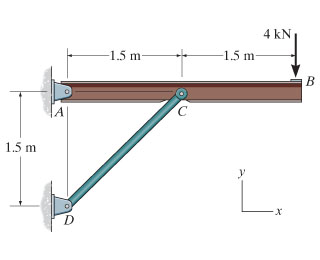
\includegraphics[width=3in]{beam.png}
\end{center}
\caption{
This is a typical example of a statics problem encountered by engineers. The goal is to understand the reactions of the pins at $A$ and $D$. \label{statics figure} Courtesy of \href{http://www.chegg.com/homework-help/questions-and-answers/draw-free-body-diagram-beam-determine-horizontal-vertical-components-beam-determine-magnit-q2963278}{chegg.com}. }
\end{figure}

To solve this type of problem, engineers apply two conservation laws.
\begin{enumerate}
 \item The first law is that the net force acting on the beam must equal the sum of individual forces acting on the beam. Since the beam is not moving (zero total net force), the sum of all forces acting on the beam is zero.  
 \item The second law is that the net torque (tendency to rotate) at every point must be zero.  Engineers use the word ``moment'' to compute torques. The process involves picking any point in the system. The moment about this point contributed by force $\vec F_i$ whose displacement from the point is $\vec d_i$ is the cross product $\vec d_i\times \vec F_i$. If we sum these torques, it must equal zero or else the rigid body will rotate.  
\end{enumerate}
Engineers spend a year practicing these ideas, and become quite fast at solving these kind of computations.  Let's walk through a computation, and then see how kernels, bases, and eigenspaces simplify the work and allow us to rapidly compute rather complex problems with ease.


\begin{problem}[Statics]
 Consider the beam diagram in Figure \ref{statics figure}. We'll first solve this exact problem for the reactions at $A$ and $D$.  Then we'll make the force $B_y$ unknown, and vary the distances. On this problem your job is to write a system of equations, and then row reduce 4 matrices. Use software. 
\begin{enumerate}
 \item The pins at $A$ and $D$ apply the forces $\vec F_A=(A_x,A_y)$ and $\vec F_D=(D_x,D_y)$ to the system consisting of the beam and rod.  The third force at $B$ is $\vec F_B=(0,B_y)=(0,-4)$ kN. Summing the forces in the $x$ direction gives the equation $A_x+D_x+0=0$. What equation do you get from summing the $y$ components? 
 \item We know $D_x=D_y$ because the rod is attached to the wall at a 45 degree angle. If instead the segment $AD$ has distance $d$ and the segment $AC$ has distance $c$, explain why $D_xd-D_yc=0$. [Think similar triangles.]  
 \item We can sum the moments about any point we choose.  The simplest point in this problem might be $C$. Summing the moments about this point gives us  $(-3/2) A_y+(3/2)B_y=0$. We now have the system of equations
$$\bvec{
1&0&1&0\\
0&1&0&1\\
0&0&1&-1\\
0&-3/2&0&0
}
\bvec{A_x\\A_y\\D_x\\D_y}
=\bvec{0\\4\\0\\(-3/2)(-4)}.$$
Solve this system to get the reactions at $A$ and $D$. 
 \item Instead of using $B_y=-4$, let's now assume that $B_y$ is an unknown force (use it as the last variable so it will become the free variable). Show how to rewrite the equation above as the homogeneous matrix equation
$$\bvec{
1&0&1&0&0\\
0&1&0&1&1\\
0&0&1&-1&0\\
0&-3/2&0&0&3/2
}
\bvec{A_x\\A_y\\D_x\\D_y\\B_y}
=\bvec{0\\0\\0\\0}.$$
Solve this system. Give a basis for kernel. If $B_y=-8$, what is $A_x$? 
 \item Continue to assume that $B_y$ is an unknown force. Let's change the distance $AD$ to be 8, the distance $AC$ to be 4, and the distance $CB$ to be 5. We can then write the system of equations as 
$$\bvec{
1&0&1&0&0\\
0&1&0&1&1\\
0&0&8&-4&0\\
0&-4&0&0&5
}
\bvec{A_x\\A_y\\D_x\\D_y\\B_y}
=\bvec{0\\0\\0\\0}.$$
Solve the system by giving a basis for the kernel. If $B_y=-8$, what is $A_x$?
\skipnow{ \item Continue to assume that $B_y$ is an unknown force. Let's change the distance $AD$ to be $d$, the distance $AC$ to be $4$, and the distance $CB$ to be $b$. We can then write the system of equations as 
$$\bvec{
1&0&1&0&0\\
0&1&0&1&1\\
0&0&d&-c&0\\
0&-c&0&0&b
}
\bvec{A_x\\A_y\\D_x\\D_y\\B_y}
=\bvec{0\\0\\0\\0}.$$
Solve the system by giving a basis for the kernel. }
\end{enumerate}
\end{problem}
%end 16





%17
%\mysubsection{\ideacon}
\subsubsection*{Kirchoff's Electrical Laws}
Gustav Kirchoff discovered two laws of electricity that pertain to the conservation of charge and energy.  To describe these laws, we must first discuss voltage, resistance, and current.  
\begin{itemize}
 \item Current is the flow of electricity. We'll often compare it to water flow or traffic flow.
 \item As a current passes across a conductor, it encounters resistance. Ohm's law states that the product of the resistance $R$ and current $I$ across a conductor equals the voltage $V$, i.e. $RI=V$. If the voltage remains constant, then a large resistance corresponds to a small current. 
 \item A resistor is an object with high resistance which is placed in an electrical system to slow down the flow (current) of electricity.  Resistors are measured in terms of ohms. The larger the ohms, the smaller the current.   
\end{itemize}
Figure \ref{ecir} illustrates two introductory electrical systems.
\begin{figure}
\begin{center}
\begin{tabular}{cc}
\renewcommand{\myscale}{.3}
\begin{tikzpicture}[scale=\myscale,inner sep=1pt]
%\draw[help lines,step=1cm] (0,0) grid (12,6);

%Source - like a battery
\node[label=right:$E$] at (0,3)
{{\begin{tikzpicture}[scale=\myscale]
%	\useasboundingbox (-.5,-3) rectangle (.5,3);
	\draw (0,0) circle (1cm);
	\draw (.3,.5) -- (-.3,.5);
	\draw (0,.2) -- (0,.8);
	\draw (.3,-.5) -- (-.3,-.5);
	\draw (0,1) -- (0,3);
	\draw (0,-1) -- (0,-3);
	\end{tikzpicture}
}};

%Resistor
\node[label=right:$R_2$] at (6,3) 
{{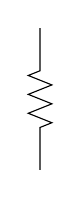
\begin{tikzpicture}[scale=\myscale]
%	\useasboundingbox (0,-3) rectangle (0,3);
	\draw (0,-3) -- ++(0,1.8) -- ++(.5,.2) 
		-- ++(-1,.4) -- ++(1,.4)
		-- ++(-1,.4) -- ++(1,.4)
		-- ++(-1,.4) -- ++(.5,.2)
		-- ++(0,1.8) ;
	\end{tikzpicture}
}};

%Resistor
\node[label=above:$R_1$] at (3,0) 
{{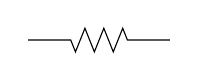
\begin{tikzpicture}[scale=\myscale,rotate=90]
%	\useasboundingbox (0,-3) rectangle (0,3);
	\draw (0,-3) -- ++(0,1.8) -- ++(.5,.2) 
		-- ++(-1,.4) -- ++(1,.4)
		-- ++(-1,.4) -- ++(1,.4)
		-- ++(-1,.4) -- ++(.5,.2)
		-- ++(0,1.8) ;
	\end{tikzpicture}
}};

%Resistor
\node[label=right:$R_3$] at (12,3) 
{{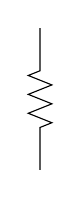
\begin{tikzpicture}[scale=\myscale,rotate=0]
%	\useasboundingbox (0,-3) rectangle (0,3);
	\draw (0,-3) -- ++(0,1.8) -- ++(.5,.2) 
		-- ++(-1,.4) -- ++(1,.4)
		-- ++(-1,.4) -- ++(1,.4)
		-- ++(-1,.4) -- ++(.5,.2)
		-- ++(0,1.8) ;
	\end{tikzpicture}
}};

%Straight Path
\node at (3,6) 
{{\begin{tikzpicture}[scale=\myscale,rotate=90]
	\draw (0,-3) -- (0,3);
	\end{tikzpicture}
}};

%Straight Path
\node at (9,6) 
{{\begin{tikzpicture}[scale=\myscale,rotate=90]
	\draw (0,-3) -- (0,3);
	\end{tikzpicture}
}};

%Straight Path
\node at (9,0) 
{{\begin{tikzpicture}[scale=\myscale,rotate=90]
	\draw (0,-3) -- (0,3);
	\end{tikzpicture}
}};


%Arrow to represent Current
\node[label=above:$i_1$] at (3,6) 
{{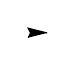
\begin{tikzpicture}[scale=\myscale,rotate=-90]
%	\useasboundingbox (0,-.4) rectangle (0,.4);
	\filldraw (0,.4) -- (-.2,-.4) -- (0,-.3) -- (.2,-.4);
	\end{tikzpicture}
}};

%Arrow to represent Current
\node[label=right:$i_2$] at (6,5) 
{{
\begin{tikzpicture}[scale=\myscale,rotate=180]
%	\useasboundingbox (0,-.4) rectangle (0,.4);
	\filldraw (0,.4) -- (-.2,-.4) -- (0,-.3) -- (.2,-.4);
	\end{tikzpicture}
}};

%Arrow to represent Current
\node[label=above:$i_3$] at (9,6) 
{{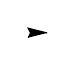
\begin{tikzpicture}[scale=\myscale,rotate=-90]
%	\useasboundingbox (0,-.4) rectangle (0,.4);
	\filldraw (0,.4) -- (-.2,-.4) -- (0,-.3) -- (.2,-.4);
	\end{tikzpicture}
}};

%Node
\node at (6,6) 
{{\begin{tikzpicture}[scale=\myscale,rotate=-90]
%	\useasboundingbox (0,-.4) rectangle (0,.4);
	\filldraw (0,0) circle (.15cm);
	\end{tikzpicture}
}};

%Node
\node at (6,0) 
{{\begin{tikzpicture}[scale=\myscale,rotate=-90]
%	\useasboundingbox (0,-.4) rectangle (0,.4);
	\filldraw (0,0) circle (.15cm);
	\end{tikzpicture}
}};

\end{tikzpicture}

&
\renewcommand{\myscale}{.3}
\begin{tikzpicture}[scale=\myscale,inner sep=1pt]
%\draw[help lines,step=1cm] (0,0) grid (18,6);

%Source - like a battery
\node[label=right:$E$] at (0,3) 
{{\begin{tikzpicture}[scale=\myscale]
%	\useasboundingbox (-.5,-3) rectangle (.5,3);
	\draw (0,0) circle (1cm);
	\draw (.3,.5) -- (-.3,.5);
	\draw (0,.2) -- (0,.8);
	\draw (.3,-.5) -- (-.3,-.5);
	\draw (0,1) -- (0,3);
	\draw (0,-1) -- (0,-3);
	\end{tikzpicture}
}};

%Resistor
\node[label=right:$R_2$] at (6,3) 
{{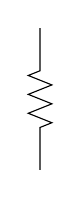
\begin{tikzpicture}[scale=\myscale]
%	\useasboundingbox (0,-3) rectangle (0,3);
	\draw (0,-3) -- ++(0,1.8) -- ++(.5,.2) 
		-- ++(-1,.4) -- ++(1,.4)
		-- ++(-1,.4) -- ++(1,.4)
		-- ++(-1,.4) -- ++(.5,.2)
		-- ++(0,1.8) ;
	\end{tikzpicture}
}};

%Resistor
\node[label=above:$R_1$] at (3,0) 
{{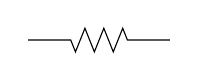
\begin{tikzpicture}[scale=\myscale,rotate=90]
%	\useasboundingbox (0,-3) rectangle (0,3);
	\draw (0,-3) -- ++(0,1.8) -- ++(.5,.2) 
		-- ++(-1,.4) -- ++(1,.4)
		-- ++(-1,.4) -- ++(1,.4)
		-- ++(-1,.4) -- ++(.5,.2)
		-- ++(0,1.8) ;
	\end{tikzpicture}
}};

%Resistor
\node[label=above:$R_3$] at (9,6) 
{{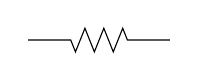
\begin{tikzpicture}[scale=\myscale,rotate=90]
%	\useasboundingbox (0,-3) rectangle (0,3);
	\draw (0,-3) -- ++(0,1.8) -- ++(.5,.2) 
		-- ++(-1,.4) -- ++(1,.4)
		-- ++(-1,.4) -- ++(1,.4)
		-- ++(-1,.4) -- ++(.5,.2)
		-- ++(0,1.8) ;
	\end{tikzpicture}
}};

%Resistor
\node[label=right:$R_4$] at (12,3) 
{{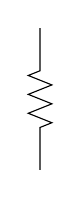
\begin{tikzpicture}[scale=\myscale,rotate=0]
%	\useasboundingbox (0,-3) rectangle (0,3);
	\draw (0,-3) -- ++(0,1.8) -- ++(.5,.2) 
		-- ++(-1,.4) -- ++(1,.4)
		-- ++(-1,.4) -- ++(1,.4)
		-- ++(-1,.4) -- ++(.5,.2)
		-- ++(0,1.8) ;
	\end{tikzpicture}
}};

%Resistor
\node[label=right:$R_5$] at (18,3) 
{{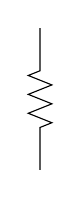
\begin{tikzpicture}[scale=\myscale,rotate=0]
%	\useasboundingbox (0,-3) rectangle (0,3);
	\draw (0,-3) -- ++(0,1.8) -- ++(.5,.2) 
		-- ++(-1,.4) -- ++(1,.4)
		-- ++(-1,.4) -- ++(1,.4)
		-- ++(-1,.4) -- ++(.5,.2)
		-- ++(0,1.8) ;
	\end{tikzpicture}
}};

%Resistor
\node[label=above:$R_6$] at (9,0) 
{{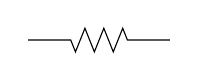
\begin{tikzpicture}[scale=\myscale,rotate=90]
%	\useasboundingbox (0,-3) rectangle (0,3);
	\draw (0,-3) -- ++(0,1.8) -- ++(.5,.2) 
		-- ++(-1,.4) -- ++(1,.4)
		-- ++(-1,.4) -- ++(1,.4)
		-- ++(-1,.4) -- ++(.5,.2)
		-- ++(0,1.8) ;
	\end{tikzpicture}
}};









%Straight Path
\node at (3,6) 
{{\begin{tikzpicture}[scale=\myscale,rotate=90]
	\draw (0,-3) -- (0,3);
	\end{tikzpicture}
}};

%Straight Path
\node at (15,6) 
{{\begin{tikzpicture}[scale=\myscale,rotate=90]
	\draw (0,-3) -- (0,3);
	\end{tikzpicture}
}};

%Straight Path
\node at (15,0) 
{{\begin{tikzpicture}[scale=\myscale,rotate=90]
	\draw (0,-3) -- (0,3);
	\end{tikzpicture}
}};






%Arrow to represent Current
\node[label=above:$i_1$] at (3,6) 
{{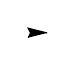
\begin{tikzpicture}[scale=\myscale,rotate=-90]
%	\useasboundingbox (0,-.4) rectangle (0,.4);
	\filldraw (0,.4) -- (-.2,-.4) -- (0,-.3) -- (.2,-.4);
	\end{tikzpicture}
}};

%Arrow to represent Current
\node[label=right:$i_2$] at (6,5) 
{{
\begin{tikzpicture}[scale=\myscale,rotate=180]
%	\useasboundingbox (0,-.4) rectangle (0,.4);
	\filldraw (0,.4) -- (-.2,-.4) -- (0,-.3) -- (.2,-.4);
	\end{tikzpicture}
}};

%Arrow to represent Current
\node[label=above:$i_3$] at (7,6) 
{{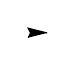
\begin{tikzpicture}[scale=\myscale,rotate=-90]
%	\useasboundingbox (0,-.4) rectangle (0,.4);
	\filldraw (0,.4) -- (-.2,-.4) -- (0,-.3) -- (.2,-.4);
	\end{tikzpicture}
}};

%Arrow to represent Current
\node[label=right:$i_4$] at (12,5) 
{{
\begin{tikzpicture}[scale=\myscale,rotate=180]
%	\useasboundingbox (0,-.4) rectangle (0,.4);
	\filldraw (0,.4) -- (-.2,-.4) -- (0,-.3) -- (.2,-.4);
	\end{tikzpicture}
}};

%Arrow to represent Current
\node[label=above:$i_5$] at (15,6) 
{{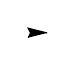
\begin{tikzpicture}[scale=\myscale,rotate=-90]
%	\useasboundingbox (0,-.4) rectangle (0,.4);
	\filldraw (0,.4) -- (-.2,-.4) -- (0,-.3) -- (.2,-.4);
	\end{tikzpicture}
}};

%Arrow to represent Current
\node[label=above:$i_6$] at (11,0) 
{{
\begin{tikzpicture}[scale=\myscale,rotate=90]
%	\useasboundingbox (0,-.4) rectangle (0,.4);
	\filldraw (0,.4) -- (-.2,-.4) -- (0,-.3) -- (.2,-.4);
	\end{tikzpicture}
}};








%Node
\node at (6,6) 
{{\begin{tikzpicture}[scale=\myscale,rotate=-90]
%	\useasboundingbox (0,-.4) rectangle (0,.4);
	\filldraw (0,0) circle (.15cm);
	\end{tikzpicture}
}};

%Node
\node at (6,0) 
{{\begin{tikzpicture}[scale=\myscale,rotate=-90]
%	\useasboundingbox (0,-.4) rectangle (0,.4);
	\filldraw (0,0) circle (.15cm);
	\end{tikzpicture}
}};

%Node
\node at (12,0) 
{{\begin{tikzpicture}[scale=\myscale,rotate=-90]
%	\useasboundingbox (0,-.4) rectangle (0,.4);
	\filldraw (0,0) circle (.15cm);
	\end{tikzpicture}
}};

%Node
\node at (12,6) 
{{\begin{tikzpicture}[scale=\myscale,rotate=-90]
%	\useasboundingbox (0,-.4) rectangle (0,.4);
	\filldraw (0,0) circle (.15cm);
	\end{tikzpicture}
}};

\end{tikzpicture}

\\
Two Loop System & Three Loop System
\end{tabular}\end{center}
\caption{Electrical Circuit Diagrams.\label{ecir}}
\end{figure}
In this diagram, wires meet at nodes (illustrated with a dot).  
Batteries and voltage sources (represented by 
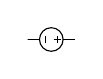
\begin{tikzpicture}[scale=.15,rotate=-90]
%	\useasboundingbox (-.5,-3) rectangle (.5,3);
	\clip (-1,-2) rectangle (1,2);
	\draw (0,0) circle (1cm);
	\draw (.3,.5) -- (-.3,.5);
	\draw (0,.2) -- (0,.8);
	\draw (.3,-.5) -- (-.3,-.5);
	\draw (0,1) -- (0,3);
	\draw (0,-1) -- (0,-3);
\end{tikzpicture}
or other symbols)
supply a voltage of $E$ volts.  At each node the current may change, so the arrows and letters $i$ represent the different currents in the electrical system. The electrical current on each wire may or may not follow the arrows drawn (a negative current means that the current flows opposite the arrow). Resistors are depicted with the symbol 	
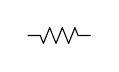
\begin{tikzpicture}[scale=.2,rotate=90]
%	\useasboundingbox (0,-3) rectangle (0,3);
	\clip (-.5,-2) rectangle (.5,2);
	\draw (0,-3) -- ++(0,1.8) -- ++(.5,.2) 
		-- ++(-1,.4) -- ++(1,.4)
		-- ++(-1,.4) -- ++(1,.4)
		-- ++(-1,.4) -- ++(.5,.2)
		-- ++(0,1.8) ;
	\end{tikzpicture}
, and the letter $R$ represents the ohms. 

Kirchoff discovered two laws. They both help us find current in a system, provided we know the voltage of any batteries, and the resistance of any resistors. 
\begin{enumerate}
	\item Kirchoff's current law states that at every node, the current flowing in equals the current flowing out (at nodes, current in = current out). 
	\item Kirchoff's voltage law states that on any loop in the system, the directed sum of voltages supplied equals the directed sum of voltage drops (in loops, voltage in = voltage out). To use this law, pick a spot in the system.  Then move around the system following a path that eventually gets you back to where you began (a closed curve). If you encounter a battery (a voltage source), then it counts as voltage in.  If you encounter a resistor as you move with the current, then the voltage drop is $Ri$.  If you encounter a resistor while moving opposite the current, then times by a negative to get a voltage drop of $-R_i$.
\end{enumerate}

Let's use Kirchoff's laws to generate a system of equations for the two loop system. Remember that every time a current encounters a resistor, the voltage drop is $V=RI$, the product of the resistance and the current. 
\begin{problem} \label{kirchoff 2 loop general}
Consider the two loop system in figure \ref{ecir}. Assume that the voltage supplied from the battery $E$, as well as the ohms $R_1$, $R_2$, and $R_3$, on the resistors are known. The currents $i_1$, $i_2$, and $i_3$ are unknown.
\begin{enumerate}
 \item Use Kirchoff's laws to explain how to obtain each of the equations below:
$$
\begin{array}{rl}
i_1-i_2-i_3&=0\\
-i_1+i_2+i_3&=0\\
R_1i_1+R_2i_2-E&=0\\
-R_2 i_2 +R_3i_3&=0.\\
R_1i_1 + R_3i_3-E&=0.
\end{array}
%\quad \Rightarrow
%\bvec{
%1&-1&-1&0\\
%-1&1&1&0\\
%R_1&R_2&0&-1\\
%0&-R_2&R_3&0\\
%R_1&0&R_3&-1
%}
%\bvec{i_1\\i_2\\i_3\\E}
%=\bvec{0\\0\\0\\0\\0}
$$
[Hint: If you encounter a resistor while moving backwards along a loop, then the voltage drop becomes a voltage gain (times by a negative).]
 \item Some of the equations above are linear combinations of the other equations.  How could you obtain the 2nd and 5th as a linear combination of the others?
 \item Suppose $R_1 = 2$, $R_2 = 3$, and  $R_3 = 6$ ohms.  Solve the system of equations above by row reducing an appropriate matrix (think of $E$ as an unknown and find the kernel of a matrix).  State a basis for the solutions.
 \item If we know the power source is $E=12$ V, what is $i_1$?  If we measure the current in the first wire to be $i_1=10$ amps, then what is $E$?
\end{enumerate}
\end{problem}
%end 17













%18
\mysubsection{\ideapro}
When we want to find the coefficients of an equation such as $y=mx+b$ or $y=ax^2+bx+c$ that passes through several points, remember that the key idea is to write the linear system of equations $A\vec x=\vec b$ that we wish to solve.  If the equation has no solution, then we multiply both sides by $A^T$ and then solve the corresponding system.  This gets us the linear combination of the columns of $A$ that is closest to $\vec b$. We call this linear regression. 
%Change this to just 5 points through a parabola.
\begin{problem}
 Consider the 5 points 
$$ 
(-1,  1),
( 0, -1),
( 1, -2),
( 2, -1),
( 2, -2)
$$
\begin{enumerate}
 \item Use linear regression to give an equation of the line $y=a_0+a_1x$ that best fits these 5 points. (Remember to set up the system $A\vec x = \vec b$, and then multiply on the left by the transpose $A^T$.) 
 \item Use linear regression to give an equation of the parabola $y=a_0+a_1x+a_2x^2$ that best fits these 5 points. 
 For this one, your system $A\vec x=\vec b$ looks like 
 $$\bvec{\nvec{1\\1\\1\\1\\1}&\nvec{-1\\0\\1\\2\\2}&\nvec{?\\?\\?\\?\\?}}\bvec{a_0\\a_1\\a_2}=\bvec{1\\-1\\-2\\-1\\-2}.$$ Just multiply both sides by $A^T$ and then solve the system of equations. The coefficients are rather ugly (one is $-115/78$).
 \item Use linear regression to give an equation of the cubic $y=a_0+a_1x+a_2x^2+a_3x^3$ that best fits these 5 points. Your answer should have some $1/12$ths in it. Graph your solution. 
 \item Why is there no quartic that passes exactly through these points?
\end{enumerate}
When you finish this problem, you should have three setups of the form $A\vec x=\vec b$. You should also show what equation you get after multiplying by $A^T$ on both sides.  Then show the rref of the resulting system, and write the equation of the line, parabola, and cubic that you obtain. 
\end{problem}
%end 18









%19
When the number of points matches the number of unknown coefficients, we can find an equation of the model without using linear regression. To organize our work, let's first standardize the notation.  Rather than writing $y=mx+b$, let's write $y=a_0+a_1 x$ (where $a_0=b$ and $a_1=m$). For a parabola, let's write $\ds y=a_0 + a_1 x+ a_2 x^2 = \sum_{k=0}^{2} a_k x^k$. We can now write any polynomial in the form $$\ds y = a_0 + a_1 x+ \cdots + a_n x^n = \sum_{k=0}^n a_k x^k.$$ By standardizing the coefficients, we can use summation notation to express any degree polynomial by changing the $n$ on the top of the summation sign. 

%\mysubsection{\ideapro}
%Way too long.  Just shave off a few parts, and this would be perfect.  The engineers didn't struggle with this problem any.  It might be a better problem at the opening.
\begin{problem}
 Answer the following by row reducing an appropriate matrix (just use software). [Hint: Each point produces an equation.]
\begin{enumerate}
 \item 
Find the intercept $a_0$ and slope $a_1$ of a line $y = a_0+a_1 x$ that passes through the points $(1,2)$ and $(3,5)$. [We could have used $m$ and $b$, but I chose to use $a_0$ and $a_1$ so we can see how this generalizes to all dimensions.]
 \item 
Find the coefficients $a_0$, $a_1$, and $a_2$ of a parabola $y = a_0+a_1 x^1+a_2x^2$ that passes through the points $(0, 1)$,  $(2, 3)$, and  $(−1, 4)$. [Hint: The second point produces the equation $3=a_0+a_1(2)+a_2(2)^2$.]
 \item
Give an equation of a cubic polynomial $y = a_0+a_1x^1+a_2x^2+a_3x^3$ that passes through the four points $(0, 1)$, $(1, 3)$, $(−1, 4)$, and $(2, 4)$. [You should have a linear system with 4 equations and 4 unknowns.]
\item 
Suppose that we collect the 6 data points $(1,1)$, $(2,3)$, $(-1,2)$, $(0,-1)$, $(-2,0)$, $(3,1)$, and we would like to find a polynomial that passes through all 6 points. State the degree $n$ of this polynomial. Then find the coefficients $a_0, a_1, \ldots, a_n$ of this polynomial. Use technology to do your row reduction.  When you present in class, show us the matrix you entered into a computer, and then show us the reduced row echelon form together with the polynomial.
\end{enumerate}
\end{problem}
%end 19













\mysubsection{\idealin}


%20
\subsubsection*{Cramer's Rule}
Gabriel Cramer developed a way to solve linear systems of equations by using determinants. For small systems, the solution is extremely fast.  For large systems the method looses its power because of the complexity of computing determinants.  However, when the coefficients in the system are variables, Cramer's rule provides an extremely fast algorithm for obtaining solutions. I'll remind you occasionally throughout the problem set to apply Cramer's rule when the problem involves variable coefficients.
\begin{problem}[Cramer's Rule]
Our goal on this problem is to find a quick way to solve the matrix equation $$\begin{bmatrix}\nvec{a_{11}\\a_{21}}&\nvec{a_{12}\\a_{22}} \end{bmatrix}
\begin{bmatrix}\nvec{x_{1}\\x_{2}} \end{bmatrix}
=
\begin{bmatrix}\nvec{b_{1}\\b_{2}} \end{bmatrix}.$$ 
Let's look at an example and from it develop a general rule. 
Let $\vec v_1 = (a_{11},a_{21})=(2,-2)$ and $\vec v_2 = (a_{12},a_{22})= (1,2)$, so $A=\bvec{2&1\\-2&2}$. If we know that $x_1=-3$ and $x_2 = -2$, the we have $\vec b = x_1\vec v_1+x_2\vec v_2=(-8,2)$. In the picture below, the solid red vector is $\vec v_1$, the solid blue vector is $\vec v_2$, and the solid black vector is $\vec b$. Use the picture below, to answer the questions that follow.

%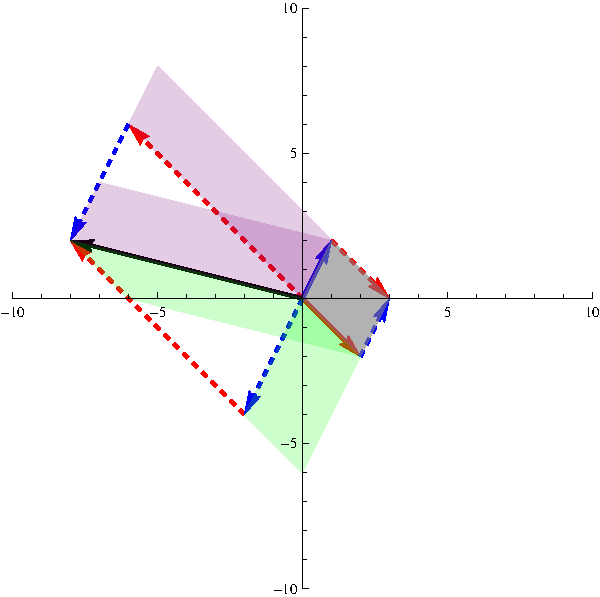
\includegraphics{cramers-visual}

\begin{center}
 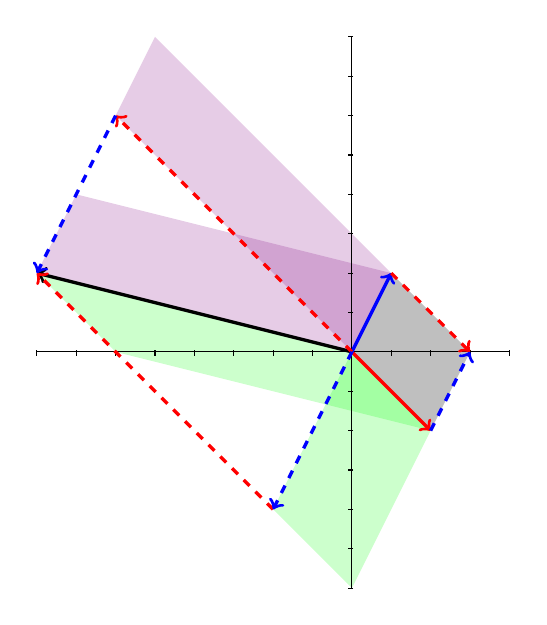
\begin{tikzpicture}[scale=.5]
  \fill[lightgray] (0,0) -- (2,-2) -- (3,0) -- (1,2) -- (0,0);
  \fill[color=red!50!blue,opacity=0.2] (0,0) -- ++(1,2) -- ++(-6,6) -- ++(-1,-2) -- ++(6,-6);
  \fill[color=red!50!blue,opacity=0.2] (0,0) -- ++(1,2) -- ++(-8,2) -- ++(-1,-2) -- ++(8,-2);
  \fill[color=green,opacity=0.2] (0,0) -- ++(2,-2) -- ++(-8,2) -- ++(-2,2) -- ++(8,-2);
  \fill[color=green,opacity=0.2] (0,0) -- ++(2,-2) -- ++(-2,-4) -- ++(-2,2) -- ++(2,4);
  %axis
  \draw (-8,0) -- coordinate (x axis mid) (4,0);
  \draw (0,-6) -- coordinate (y axis mid) (0,8);
  %ticks
  \foreach \x in {-8,...,4}
   \draw (\x,1pt) -- (\x,-3pt)
    node[anchor=north] {};
  \foreach \y in {-6,...,8}
   \draw (1pt,\y) -- (-3pt,\y) 
    node[anchor=east] {}; 
  \draw[red,->,very thick] (0,0) -- (2,-2);
  \draw[blue,->,very thick] (0,0) -- (1,2);
  \draw[black,->,very thick] (0,0) -- (-8,2);
  \draw[red,->,very thick,dashed] (1,2) -- ++(2,-2);
  \draw[blue,->,very thick,dashed] (2,-2) -- ++(1,2);
  \draw[red,->,very thick,dashed] (0,0) -- ++(-6,6);
  \draw[red,->,very thick,dashed] (-2,-4) -- ++(-6,6);
  \draw[blue,->,very thick,dashed] (0,0) -- ++(-2,-4);
  \draw[blue,->,very thick,dashed] (-6,6) -- ++(-2,-4);
 \end{tikzpicture}
\end{center}


\noindent[Hint: Each question can be answered by thinking about determinants as areas.]
\begin{enumerate}
 \item 
 \marginpar{Remember that when we put vertical bars on a matrix, that means we compute the determinant.}%
 Explain why $x_1\begin{vmatrix}\vec{v_1}&\vec v_2\end{vmatrix}=\begin{vmatrix}x_1\vec{v_1}&\vec v_2\end{vmatrix}$.  
\item Now explain why $\begin{vmatrix}x_1\vec{v_1}&\vec v_2\end{vmatrix} = \begin{vmatrix}\vec{b}&\vec v_2\end{vmatrix}$. [Hint: Why do the two purple parallelograms have the same area?]  
 \item Finally, solve for $x_1$ to show that $$x_1 = \frac{\begin{vmatrix}\nvec{b_1\\b_2}&\nvec{a_{12}\\a_{22}} \end{vmatrix}}{\begin{vmatrix}\nvec{a_{11}\\a_{21}}&\nvec{a_{12}\\a_{22}} \end{vmatrix}}.$$
 \item In a similar fashion, show that $$x_2 =\frac{\begin{vmatrix}\nvec{a_{11}\\a_{21}}&\nvec{b_1\\b_2}\end{vmatrix}}{\begin{vmatrix}\nvec{a_{11}\\a_{21}}&\nvec{a_{12}\\a_{22}} \end{vmatrix}}.$$ 
 \item Consider the system of equations $x+2y=3, 4x+5y=6$. Use the formulas you just developed to solve this system. You'll need to compute three determinants.
 \end{enumerate}
\end{problem}




The previous problem is a proof by picture of Cramer's rule in 2D. The proof of the theorem is similar in all dimensions. The key idea is to connect determinants to area.  
Here's a formal statement of Cramer's Rule.
\begin{theorem}[Cramer's Rule]\label{Cramer's Rule}
 Consider the linear system given by $A\vec x = \vec b$, where 
$A=\begin{bmatrix}\vec v_1 &\vec v_2 &\cdots \vec v_n \end{bmatrix}$
is an $n$ by $n$ matrix whose determinant is not zero.  Let $D=|A|$. For each $i$, replace vector $\vec v_i$ with $\vec b$, and then let $D_i$ be the determinant of the corresponding matrix. The solution to the linear system is
$$x_1 = \frac{D_1}{D},\quad x_2 = \frac{D_2}{D},\quad \cdots \quad x_n = \frac{D_n}{D}.$$

For the 2 by 2 system
$$
\begin{bmatrix}\nvec{a_{11}\\a_{21}}&\nvec{a_{12}\\a_{22}} \end{bmatrix}
\begin{bmatrix}\nvec{x_{1}\\x_{2}} \end{bmatrix}
=
\begin{bmatrix}\nvec{b_{1}\\b_{2}} \end{bmatrix},
$$
Cramer's rule states the solution is (provided $|A|\neq 0$) 
$$
x_1 = \frac{D_1}{D}=\frac{\begin{vmatrix}\nvec{b_1\\b_2}&\nvec{a_{12}\\a_{22}} \end{vmatrix}}{\begin{vmatrix}\nvec{a_{11}\\a_{21}}&\nvec{a_{12}\\a_{22}} \end{vmatrix}},
\quad 
x_2 = \frac{D_2}{D}=\frac{\begin{vmatrix}\nvec{a_{11}\\a_{21}}&\nvec{b_1\\b_2}\end{vmatrix}}{\begin{vmatrix}\nvec{a_{11}\\a_{21}}&\nvec{a_{12}\\a_{22}} \end{vmatrix}}
.$$
\end{theorem}
%end 20











%21
\mysubsection{\ideapro}
\begin{problem}
Solve the following. [Hint: Because the problem involves variable points, Cramer's rule will be much faster than row reduction.]
\begin{enumerate}
 \item Find the intercept $a_0$ and slope $a_1$ of a line $y = a_0+a_1 x$ that passes through the points $(x_1,y_1)$ and $(x_2,y_2)$. 
 \item Use Cramer's rule to state the coefficients $a_1$ of a parabola $y = a_0+a_1 x^1+a_2x^2$ that passes through the points $(x_1, y_1)$,  $(x_2, y_2)$, and  $(x_3, y_3)$. You could similarly find $a_0$ and $a_2$, but don't worry about it.
\end{enumerate}
Can you think of any conditions where your solutions above will not be valid?
\end{problem}
%end 21













%22
%\mysubsection{\ideapro}

We've seen how to linear regression to find an equation of lines, parabolas, cubics, and more that best fit several data points. The key is to set up a system which has no solution, multiply both sides on the left by the transpose, and then solve. Let's use this idea to obtain a general solution for finding an equation of the linear regression line that best approximates some arbitrary points. 

%Do 5 points through a line.  Leave them general.
\begin{problem}
 Consider the five points 
 $$
 (x_1,y_1),
 (x_2,y_2),
 (x_3,y_3),
 (x_4,y_4),
 (x_5,y_5).
$$
We would like to find an equation of the least squares regression line $y=a_0+a_1x$ that best fits these points. 
Set up the matrices $A$, $\vec x$, $\vec b$, and $A^T$. Multiply together $A^TA$ and $A^T\vec b$ (your result should involve sums of the form $\sum x_i$, $\sum y_i$, $\sum x_iy_i$, and $\sum x_i^2$). Then solve the equation $A^TA\vec x = A^T\vec b$ and state the coefficients $a_0$ and $a_1$. 

[Hint: Since the system involves variable coefficients, try using Cramer's rule. It should kick out the solution almost instantly with 3 two by two determinants. One of these determinants should be $(5)\left(\sum x_iy_i\right) - \left(\sum x_i\right)\left(\sum y_i\right)$.]
\end{problem}

The formula you developed above is the formula found in software programs.  It's also the formula you'll find in statistic textbooks, high school textbooks, online help sites, etc.  They just change the $5$ to an $n$. 
% This concept is one that you can help students in high school understand.  Most books just say, ``Multiply by $A^T$,'' but never give a reason why you would do that.  You can help students understand that $A\vec x$ is a linear combination of the columns of $A$, and that regression just asks them to find the linear combination that gets them closest to $\vec b$. 
%end 22





%\end{document}



\skipnow{


%23
\mysubsection{\ideanon}
\subsubsection*{The Arms Race}
%Cramer's rule is most useful when the coefficients in the linear system are variables, rather than numbers.  
Let's apply our knowledge to study the arms race (the building of armies - tanks, bombs, soldiers, etc. - between two countries).  Consider two countries, country $A$ and country $B$. As country $B$ builds up their military, country $A$ looks on and says ``Hmm, we better build up our military.''  Similarly, as country $A$ builds up their military, country $B$ says the same. If country $A$ has a grudge against country $B$, they will probably build up their military regardless of what country $B$ does.  Similarly, any past grievances and grudges that country $B$ has against country $A$ will increase the rate at which country $B$ builds up their military. Building up a military costs money, so hopefully both countries have economic limitations that restrict the growth of their military. The real question behind the arms race is,
\begin{quote}
 Will the two countries eventually decide they are spending enough on their military, or will their spending continue to grow without bound.
\end{quote}

 We now develop a system of differential equations that describes the above. We've seen the idea ``flow in equals flow out'' in our conservation problems.  In this case, arms are not conserved.  Instead, we have the following rule:
\begin{quote}
 The change in a quantity equals the flow in of the quantity minus the flow out of the quantity, or more simply 
$$\text{Change = (Flow in) - (Flow out)}$$
$$\text{Change = (Increase) - (Decrease)}$$
\end{quote}
\begin{itemize}
\item Let $x$ represent the dollar amount per year that country $A$ spends on arms. Let $y$ represent the dollar amount per year that country $B$ spends on arms.  
\item When $y$ is large, country $A$ will respond by increasing their spending.  
We'll assume this change is proportional to $y$, so we see that $x$ increases by an amount $ay$. 
 Similarly, when $x$ is large, country $B$ responds by increasing their spending. Let's assume that $y$ increases by an amount $mx$.
\item The economy of each country tries to slow down the spending rate.  The more money country $A$ spends, the larger the effect of the economy.  We'll assume that $x$ decreases by an amount proportional to itself, namely $bx$.  Similarly, we'll assume $y$ decrease by an amount $ny$.
\item If the countries hold grudges against each other for past grievances, then they are inclined to increase their spending regardless of economic factors and the growth of the other country's army.  Let $c$ represent the amount that country $A$ will increase their spending by, and let $p$ represent the amount that country $B$ will increase their spending by. These values might be zero (for example the US and Canada do not hold such grudges), but might not be zero at all (as was the case during the cold war, between the US and USSR).
\end{itemize}

\begin{problem}
Start by reading the arms race information above.
\begin{enumerate}
 \item There are three things causing $x$ to change. The flow in (parts causing an increase) are $ay$, the response to the other country, and $c$, any grudges.  The flow out (parts causing a decrease) is only $bx$, the economic restriction.  We can write this as a differential equation $$\frac{dx}{dt} = ay+c-bx.$$ Obtain a similar equation for $\dfrac{dy}{dt}$ (using the coefficients $m$, $n$, and $p$). Then write your system of ODEs in the form 
$$
\begin{bmatrix}x'\\y'\end{bmatrix}
=
\begin{bmatrix}-b&a\\?&?\end{bmatrix}
\begin{bmatrix}x\\y\end{bmatrix}
+
\begin{bmatrix}c\\?\end{bmatrix}.
$$ 
 \item An equilibrium solution to the system of differential equations above is a solution that remains stable (flow in equals flow out). At equilibrium, there should not be any future change in $x$ nor $y$, so we should have $dx/dt=0$ and $dy/dt=0$. Find the equilibrium solution for the arms race problem. [Cramer's rule should make this really fast.]
 \item We can write the differential equation in vector field form as $(x',y') = (ay+c-bx,...)$.  Compute the derivative of this vector field to obtain a 2 by 2 matrix.  
 \item Find the eigenvalues of this matrix. [Use the quadratic formula.] 
 \item (Challenge) If any eigenvalue of this matrix is positive, then uncontrolled spending will occur. What conditions must be met so that both eigenvalues are not positive?
%In class, we'll pick some positive values for $a,b,c,m,n,p$ that satisfy the conditions you tell us, and then graph the vector field $\frac{d \vec x}{dt} = A\vec x+\vec p$, along with some solution curves.  
\end{enumerate}
\end{problem}
%end 23

}







\mysubsection{\ideacon}
Let's return to another problem involving Kirchoff's electrical laws. 

%24
%Change this.  Make sure it puts $E$ as a column in the matrix. 
\begin{problem}
Consider the three loop system below. 
\begin{center}
\renewcommand{\myscale}{.3}
\begin{tikzpicture}[scale=\myscale,inner sep=1pt]
%\draw[help lines,step=1cm] (0,0) grid (18,6);

%Source - like a battery
\node[label=right:$E$] at (0,3) 
{{\begin{tikzpicture}[scale=\myscale]
%	\useasboundingbox (-.5,-3) rectangle (.5,3);
	\draw (0,0) circle (1cm);
	\draw (.3,.5) -- (-.3,.5);
	\draw (0,.2) -- (0,.8);
	\draw (.3,-.5) -- (-.3,-.5);
	\draw (0,1) -- (0,3);
	\draw (0,-1) -- (0,-3);
	\end{tikzpicture}
}};

%Resistor
\node[label=right:$R_2$] at (6,3) 
{{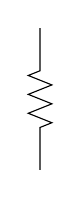
\begin{tikzpicture}[scale=\myscale]
%	\useasboundingbox (0,-3) rectangle (0,3);
	\draw (0,-3) -- ++(0,1.8) -- ++(.5,.2) 
		-- ++(-1,.4) -- ++(1,.4)
		-- ++(-1,.4) -- ++(1,.4)
		-- ++(-1,.4) -- ++(.5,.2)
		-- ++(0,1.8) ;
	\end{tikzpicture}
}};

%Resistor
\node[label=above:$R_1$] at (3,0) 
{{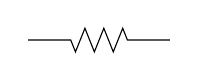
\begin{tikzpicture}[scale=\myscale,rotate=90]
%	\useasboundingbox (0,-3) rectangle (0,3);
	\draw (0,-3) -- ++(0,1.8) -- ++(.5,.2) 
		-- ++(-1,.4) -- ++(1,.4)
		-- ++(-1,.4) -- ++(1,.4)
		-- ++(-1,.4) -- ++(.5,.2)
		-- ++(0,1.8) ;
	\end{tikzpicture}
}};

%Resistor
\node[label=above:$R_3$] at (9,6) 
{{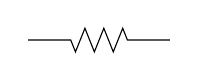
\begin{tikzpicture}[scale=\myscale,rotate=90]
%	\useasboundingbox (0,-3) rectangle (0,3);
	\draw (0,-3) -- ++(0,1.8) -- ++(.5,.2) 
		-- ++(-1,.4) -- ++(1,.4)
		-- ++(-1,.4) -- ++(1,.4)
		-- ++(-1,.4) -- ++(.5,.2)
		-- ++(0,1.8) ;
	\end{tikzpicture}
}};

%Resistor
\node[label=right:$R_4$] at (12,3) 
{{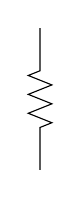
\begin{tikzpicture}[scale=\myscale,rotate=0]
%	\useasboundingbox (0,-3) rectangle (0,3);
	\draw (0,-3) -- ++(0,1.8) -- ++(.5,.2) 
		-- ++(-1,.4) -- ++(1,.4)
		-- ++(-1,.4) -- ++(1,.4)
		-- ++(-1,.4) -- ++(.5,.2)
		-- ++(0,1.8) ;
	\end{tikzpicture}
}};

%Resistor
\node[label=right:$R_5$] at (18,3) 
{{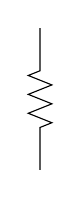
\begin{tikzpicture}[scale=\myscale,rotate=0]
%	\useasboundingbox (0,-3) rectangle (0,3);
	\draw (0,-3) -- ++(0,1.8) -- ++(.5,.2) 
		-- ++(-1,.4) -- ++(1,.4)
		-- ++(-1,.4) -- ++(1,.4)
		-- ++(-1,.4) -- ++(.5,.2)
		-- ++(0,1.8) ;
	\end{tikzpicture}
}};

%Resistor
\node[label=above:$R_6$] at (9,0) 
{{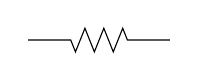
\begin{tikzpicture}[scale=\myscale,rotate=90]
%	\useasboundingbox (0,-3) rectangle (0,3);
	\draw (0,-3) -- ++(0,1.8) -- ++(.5,.2) 
		-- ++(-1,.4) -- ++(1,.4)
		-- ++(-1,.4) -- ++(1,.4)
		-- ++(-1,.4) -- ++(.5,.2)
		-- ++(0,1.8) ;
	\end{tikzpicture}
}};









%Straight Path
\node at (3,6) 
{{\begin{tikzpicture}[scale=\myscale,rotate=90]
	\draw (0,-3) -- (0,3);
	\end{tikzpicture}
}};

%Straight Path
\node at (15,6) 
{{\begin{tikzpicture}[scale=\myscale,rotate=90]
	\draw (0,-3) -- (0,3);
	\end{tikzpicture}
}};

%Straight Path
\node at (15,0) 
{{\begin{tikzpicture}[scale=\myscale,rotate=90]
	\draw (0,-3) -- (0,3);
	\end{tikzpicture}
}};






%Arrow to represent Current
\node[label=above:$i_1$] at (3,6) 
{{\begin{tikzpicture}[scale=\myscale,rotate=-90]
%	\useasboundingbox (0,-.4) rectangle (0,.4);
	\filldraw (0,.4) -- (-.2,-.4) -- (0,-.3) -- (.2,-.4);
	\end{tikzpicture}
}};

%Arrow to represent Current
\node[label=right:$i_2$] at (6,5) 
{{\begin{tikzpicture}[scale=\myscale,rotate=180]
%	\useasboundingbox (0,-.4) rectangle (0,.4);
	\filldraw (0,.4) -- (-.2,-.4) -- (0,-.3) -- (.2,-.4);
	\end{tikzpicture}
}};

%Arrow to represent Current
\node[label=above:$i_3$] at (7,6) 
{{\begin{tikzpicture}[scale=\myscale,rotate=-90]
%	\useasboundingbox (0,-.4) rectangle (0,.4);
	\filldraw (0,.4) -- (-.2,-.4) -- (0,-.3) -- (.2,-.4);
	\end{tikzpicture}
}};

%Arrow to represent Current
\node[label=right:$i_4$] at (12,5) 
{{\begin{tikzpicture}[scale=\myscale,rotate=180]
%	\useasboundingbox (0,-.4) rectangle (0,.4);
	\filldraw (0,.4) -- (-.2,-.4) -- (0,-.3) -- (.2,-.4);
	\end{tikzpicture}
}};

%Arrow to represent Current
\node[label=above:$i_5$] at (15,6) 
{{\begin{tikzpicture}[scale=\myscale,rotate=-90]
%	\useasboundingbox (0,-.4) rectangle (0,.4);
	\filldraw (0,.4) -- (-.2,-.4) -- (0,-.3) -- (.2,-.4);
	\end{tikzpicture}
}};

%Arrow to represent Current
\node[label=above:$i_6$] at (11,0) 
{{\begin{tikzpicture}[scale=\myscale,rotate=90]
%	\useasboundingbox (0,-.4) rectangle (0,.4);
	\filldraw (0,.4) -- (-.2,-.4) -- (0,-.3) -- (.2,-.4);
	\end{tikzpicture}
}};








%Node
\node at (6,6) 
{{\begin{tikzpicture}[scale=\myscale,rotate=-90]
%	\useasboundingbox (0,-.4) rectangle (0,.4);
	\filldraw (0,0) circle (.15cm);
	\end{tikzpicture}
}};

%Node
\node at (6,0) 
{{\begin{tikzpicture}[scale=\myscale,rotate=-90]
%	\useasboundingbox (0,-.4) rectangle (0,.4);
	\filldraw (0,0) circle (.15cm);
	\end{tikzpicture}
}};

%Node
\node at (12,0) 
{{\begin{tikzpicture}[scale=\myscale,rotate=-90]
%	\useasboundingbox (0,-.4) rectangle (0,.4);
	\filldraw (0,0) circle (.15cm);
	\end{tikzpicture}
}};

%Node
\node at (12,6) 
{{\begin{tikzpicture}[scale=\myscale,rotate=-90]
%	\useasboundingbox (0,-.4) rectangle (0,.4);
	\filldraw (0,0) circle (.15cm);
	\end{tikzpicture}
}};

\end{tikzpicture}
 
\end{center}
Assume that the voltage supplied from the battery $E$ and that the ohms $R_j$ on the resistors are known. The currents are unknown. Even though $E$ is known, treat it as an unknown so that it can act as the free variable in our final solution. 
\begin{enumerate}
 \item There are 4 nodes in this system. Write the 4 equations we obtain from Kirchoff's current law (flow in equal flow out at a node). 
 \item There are three inner loops in the system above. Write the equations formed by going around each inner loop using Kirchoff's voltage law (current in equals current out along any loop). As a reminder, here's how to get the equation from the middle loop. Start at the node in the upper left corner and move clockwise.  We encounter $R_3$ while moving with $i_3$.  We then move down $i_4$ and encounter $R_4$.  Along $i_6$ at the bottom we move left and encounter $R_6$.  We then move up (against) $i_2$ and encounter $R_2$.  Our equation is $$-R_2i_2+R_3i_3+R_4i_4+R_6i_6=0,$$ where the negative on $R_2i_2$ comes because we encountered $R_2$ while moving against the flow of $i_2$.
 \item You should have 7 equations with 7 unknowns (treating $E$ as the last unknown).  Write your system of equations in the form $A\vec x = \vec 0$.  Your matrix will have $R_i$'s in it, lots of zeros, and some 1's and $-1$'s.
%$$\begin{bmatrix}
% 1 & -1 & -1 & 0 & 0 & 0 & 0 \\
% 0 & 0 & 1 & -1 & -1 & 0 & 0 \\
% 0 & 0 & 0 & 1 & 1 & -1 & 0 \\
% -1 & 1 & 0 & 0 & 0 & 1 & 0 \\
% R_1 & R_2 & 0 & 0 & 0 & 0 & -1 \\
% 0 & -R_2 & R_3 & R_4 & 0 & R_6 & 0 \\
% 0 & 0 & 0 & -R_4 & R_5 & 0 & 0
%\end{bmatrix}
%\bvec{i_1\\i_2\\i_3\\i_4\\i_5\\i_6\\E}
%=
%\bvec{}.$$
%[Don't row reduce this matrix.]
\item If $R_1 = 1$, $R_2 = 1$, $R_3 = 1$, $R_4 = 1$, $R_5 = 1$, $R_6 = 1$, find the unknown currents by finding an eigenvector of $A$ corresponding to $\lambda = 0$ (i.e., give a basis for the eigenspace $E_A(0)$, which just means find the kernel of $A$ or just solve the system). 
 \item If $E=12$ V, what is $i_1$?  If $i_1=12$ amps, what is $E$?
\end{enumerate}
\end{problem}
%end 24






















% 25 Rewrite.......................................................
\mysubsection{\idealin}

We've been using linear combinations to organize almost all our work.  The solutions to $A\vec x = \vec b$ are always a linear combination of some vectors.  The matrix product $A\vec x$ is a linear combination of the columns of $A$.  We can use the rref of a matrix to write each column as a linear combination of the pivot columns. Once we have a basis for the kernel, every other solution is a linear combination of these basis vectors.  The list goes on.

You've been using operations that preserve linear combinations for quite some time.  This next problem has you show this.
\begin{problem}[\mynow{Optional}] Complete the following:\label{linear function examples}
\begin{enumerate}
 \item If we think of $A$ as a coordinate map $T(\vec x) = A\vec x$, then does $$A(c_1\vec x_1+c_2\vec x_2) = c_1A(\vec x_1)+c_2A(\vec x_2)?$$ Explain. (Your answer can be really short). This shows that a matrix coordinate transformation preserves linear combinations of vectors. 
 \item Explain why $\ds\frac{d}{dx}(c_1f_1(x)+c_2f_2(x)) = c_1\frac{d}{dx}(f_1)+c_2\frac{d}{dx}(f_2)$. What two differentiation rules are needed to explain why this is true?  Once you are finished, you'll have shown that the derivative operator preserves linear combinations of functions.
 \item Explain why $\ds \int_a^b c_1f_1+c_2f_2 dx = c_1\int_a^b f_1dx+c_2\int_a^b f_2dx$. Again, this shows that the integral operator preserves linear combinations of functions.
 \item Does the Laplace transform preserve linear combinations of functions?
\end{enumerate}

\end{problem}

Each of the examples above provided an example of a function, operation, or transformation that preserved linear combinations. When this occurs, we can perform the linear combination either before or after we perform the operation.  Let's make a definition to isolate this pattern. 

\begin{definition}[Function, Transformation, Operator]
 A function $f$ has a domain $D$ and range $R$. The domain $D$ is the set of inputs to the function.  The range is the set of outputs. \marginpar{The words function, transformation, and operator are all synonyms. We just typically use transformation to talk about functions when the domain is vectors, and operator to talk about functions when the domain is functions.  }%
\begin{itemize}
 \item When the domain $D$ is a collections of vectors, we'll often say that $f$ is a transformation of vectors and write $T(\vec x)$ instead of $f(x)$. An example is $T(\vec x)=A\vec x$ where $A$ is a matrix. 
 \item When the domain $D$ is a collection of functions, we'll often say that $f$ is an operator on functions and write $L(g)$ instead of $f(g)$. An example is $L(g)=\frac{d}{dx}g$ of $L(g) = \int_a^b gdx$.
\end{itemize}
\end{definition}
\begin{definition}[Linear function, Linear Transformation, Linear Operator]
 When the domain $D$ and range $R$ of a function (transformation, operator) are vector spaces (so we can perform linear combinations), then we say that the function $f$, transformation $T$, or operator $L$ is linear if it preserves linear combinations. This means that 
\begin{align*}
f(c_1x_1+c_2x_2) &= c_1f(x_1)+c_2g(x_2) \quad \text{or}\\
T(c_1\vec x_1+c_2\vec x_2) &= c_1T(\vec x_1)+c_2T(\vec x_2) \quad \text{or}\\
L(c_1 f_1+c_2 f_2) &= c_1L( f_1)+c_2L( f_2). 
\end{align*}
We can apply linear combinations either before or after we apply the function. 
\end{definition}

In problem \ref{linear function examples}, we showed that $T(\vec x)=A\vec x$ is a linear transformation and that the derivative, integral, and Laplace transform are linear operators. 
We can differentiate a sum by differentiating each piece separately (term-by-term differentiation) and we can pull constants out.  Similarly, we can integrate term-by-term, and pull constants come out.  These are precisely the key properties behind a linear function. 
\begin{quote}
If you ever find yourself saying, ``Just do each part individually,'' chances are pretty high that you are using linearity.  
\end{quote}

%end 25










%26
If $A$ is a matrix, then the product $A\vec x$ is a linear transformation.  We'll often write this as $T(\vec x) = A\vec x$. Do you remember Candice's treasure map in Problem \ref{candice's treasure}.  Once she knew how to locate 2 linearly independent object on her map (the two trees), she could translate the entire map. Once we understand how the map transforms a basis for the domain, we understand the entire linear transformation.  

\begin{problem}[\mynow{Optional}]
 Suppose that we have a linear transformation $T:\mathbb{R}^3\to \mathbb{R}^2$. Since we are mapping vectors from 3D to 2D, we could think of this as a way of portraying a three dimensional world on a flat 2D screen (so computer animation). 
 
 We've been told that $T(1,0,0) = (1,3)$, $T(0,1,0) = (-2,4)$, and that $T(1,1,1)=(3,1)$. 
\begin{enumerate}
 \item Show that $(1,0,0)$, $(0,1,0)$, and $(1,1,1)$ are a basis for $\mathbb{R}^3$. 
 \item Write $(0,0,1)$ as a linear combination of $(1,0,0)$, $(0,1,0)$, and $(1,1,1)$, and then use the fact that $T$ is linear to compute $T(0,0,1)$. 
 \item Since $(x,y,z) = (1,0,0)x+(0,1,0)y+(0,0,1)z$, and we know $T$ at each of these three vectors, compute $T(x,y,z)$. 
 \item Find a matrix $A$ so that $T(x,y,z)= A\pvec{x\\y\\z}$. 
 \item Find the kernel of the linear transformation $T$. Ask me in class to talk about what this means in terms of 3D animation.
\end{enumerate}
    
\end{problem}
%end 26

Not every function, transformation, or operator is linear. The next problem has you distinguish between a few examples.
\begin{problem}[\mynow{Optional}]
 Complete the following. When a variable is not listed as part of the domain, we assume it is constant. 
\begin{enumerate}
 \item Show that $f(x)=ax^2$ is not linear ($a$ is a constant). [Does $f(c_1x_1+c_2x_2) = c_1f(x_1)+c_2f(x_2)$?]
 \item Show that $f(a)=ax^2$ is linear ($x$ is a constant). [Does $f(c_1a_1+c_2a_2) = c_1f(a_1)+c_2f(a_2)$?]
 \item Consider $f(x)=mx+b$. Show that $f$ is not a linear function of $x$. \marginpar{Wait! So $f(x)=mx+b$ is not linear? Ask me about this in class.}%
 \item Consider $f(m,b)=mx+b$.  Show that $f$ is a linear function of $m$ and $b$. 
[Does $f(c_1(m_1,b_1)+c_2(m_2,b_2)) = c_1f(m_1,b_1)+c_2f(m_2,b_2)$?]
 \item \marginpar{This last examples explains why we use the phrase ``linear'' regression to find the coefficients of any degree polynomial that passes through some given data points.}%
Which do you think is linear, $f(x) = ax^2+bx+c$ or $f(a,b,c) = ax^2+bx+c$?
\end{enumerate}

\end{problem}
  

We'll come back to linear transformations all semester long.  We'll soon see that solving differential equations requires that we find the kernel of a linear operator. 

















%Do this only if the students are working hard.  It's an extra problem.
\mysubsection{\ideacon}
\begin{problem}[Google PageRank](Thanks to David Stowell for this problem) 
\marginpar{Many people think that we use the word PageRank because we are ranking web pages. The name comes from its creator, Larry Page. You can read more via a Google search (ironic), or with the article \href{http://epubs.siam.org/doi/abs/10.1137/050623280}{http://epubs.siam.org/doi/abs/10.1137/050623280}.}%
The Google Search Engine uses an algorithm called PageRank.
The basic idea is that the world wide web contains a number of documents with links connecting them all.  
Each document is ranked according to its importance.
A document's importance score depends on how many other pages have links pointing to it.
To fix ideas,suppose that we have four pages in our web: $P_1$, $P_2$, $P_3$, and $P_4$. 
Now suppose that this web has the following links:\
\begin{itemize}
 \item $P_1$ has outgoing links to all other pages.
 \item $P_2$ has outgoing links to $P_3$ and $P_4$.
 \item $P_3$ has outgoing links to $P_1$.
 \item $P_4$ has outgoing links to $P_1$ and $P_3$.
\end{itemize}
To determine the importance of a particular page, we simply need to count the number of times all the other pages have voted for that page.  In addition, each page has only one vote, or point, to give. It can give that one point to one page, by voting for only one page, or it can also choose to divide its vote among all the pages it votes for. In our example above, $P_1$ has two incoming links, called backlinks.
Its importance score we'll denote by $x_1$ and we compute it with $x_1 = (1){x_3}+\frac{1}{2}x_4$. Notice that the only links coming into $P_1$ are from $P_3$ and $P_4$. Moreover, $P_3$ only votes once, while $P_4$ splits its vote in two ways -- half of its vote goes to $P_1$, the other half to $P_3$. 
\begin{enumerate}
 \item Obtain an equation for $x_2$, $x_3$, and $x_4$, similar to the one above.  Then write your system of equations in the form 
$$
\bvec{
0&0&1&\frac{1}{2}\\
1/3&0&0&0\\
*&*&*&*\\
*&*&*&*
}
\bvec{x_1\\x_2\\x_3\\x_4}=\bvec{x_1\\x_2\\x_3\\x_4}.
$$
\item Look at the structure of the matrix.  In particular, what do you notice about the columns of the matrix?
\item Notice that the above equation can be written as $A\vec x = \lambda \vec x$. What is the eigenvalue $\lambda$? (If we write $y=x$, then the slope is there, even though it appears to be missing.)
\item Compute the eigenvector associated with this eigenvalue.  From your computation, which page is the most important?
\end{enumerate}
The world wide web consists of billion to trillions of pages. Modern computers can find eigenvectors of this size of a matrix extremely quickly.  
\end{problem}
%end 29
















\begin{problem}[Markov Process]
Suppose we own a car rental company which rents cars in Idaho Falls and Rexburg. 
The last few weeks have shown a weekly trend that 60\% of the cars which are rented in Rexburg will remain in Rexburg (the other 40\% end up in Idaho Falls). 
About 80\% of the cars which are rented in Idaho Falls will remain in Idaho Falls (the other 20\% end up in Rexburg). 
\begin{enumerate}
 \item If there are currently 60 cars in Rexburg and 140 cars in IF, how many will be in each city next week? If this trend continues, how many will be in each city in 2 weeks?
 \item Let $R_n$ and $I_n$ be the number of cars in Rexburg and Idaho Falls, respectively, at the beginning of the $n$th week, where $R_0=60$ and $I_0=140$. We know that we can compute $R_{n+1}$ by summing of 60\% of $R_n$ and 20\% of $I_n$. This gives us the equation $R_{n+1}=0.6 R_n+0.2I_n$. Write a similar equation for $I_{n+1}$ and then organize your work into the matrix form $$A\pvec{R_{n}\\I_{n}} = \pvec{R_{n+1}\\I_{n+1}}.$$  You can check your work by computing $A\pvec{R_0\\I_0} = \pvec{R_1\\I_1}$, which you computed above.
 \item We would like to know if the number of cars will stabilize in each city. This would mean that if the current week's car totals are $R$ and $I$, then we could find the next week's totals by solving the system $$A\pvec{R\\I} = \pvec{R\\I}.$$  The totals don't change, so we call this a steady state solution. Find the steady state solution by solving $A\pvec{R\\I} = \pvec{R\\I}$. %(What does it have to do with eigenvalues and eigenvectors?)  
 \item In the long run, what proportion of the cars will end up in Rexburg?
 \item Because the system $A\pvec{R\\I} = \pvec{R\\I}$ had a nonzero solution, we know something about the eigenvalues of the matrix $A$.  Can you spot an eigenvalue of $A$ without doing any computations?\marginpar{Recall that an eigenvalue satisfies the equation $A\vec x = \lambda \vec x$. }
\end{enumerate}
(We'll answer 4 and 5 in class if you are unable.  The key parts are 1-3.) 
\end{problem}



In the problem above, each week we could assign a car a state (Rexburg or IF).  The matrix $A$ above helped us get from one state to another.  Other examples of states are ``open'' or ``closed'' in an electrical circuit, or ``working properly'' and ``working improperly'' for operation of machinery at a manufacturing facility.  Stock market analysts use Markov processes and a generalization called stochastic processes to make predictions about future stock values. A car rental company which rents vehicles in different locations can use a Markov Process to keep track of where their inventory of cars will be in the future.  Imagine if you worked for Alamo and had thousands of car rental spots. Knowing where your cars will end up will let you know where to hire drivers, so you can move the cars to where they are needed. 









We call the matrix $A$ in a Markov process a transition matrix.  It's the matrix which tells you how to move from the current state $\vec x_n$ to the next state $\vec x_{n+1}$. This means we have 
\begin{align*}
\vec x_1 &= A\vec x_0\\
\vec x_2 &= A\vec x_1 = A(A\vec x_0) = A^2\vec x_0\\
\vec x_3 &= A\vec x_2 = A(A\vec x_1) =\cdots = A^3\vec x_0\\
\vec x_4 &= A\vec x_3 = A(A\vec x_2) =\cdots = A^4\vec x_0\\
&\vdots
\end{align*}
You can find the $n$th state by computing $\vec x_n = A^n \vec x_0$. We just raise the matrix to a power, and times by the initial state. The next problem has you examine what happens when you raise a matrix to a power. 
%Here is a perfect spot to talk about why eigenvalues are so important, and why having an eigenvalue of 1 is also so crucial. If I could get to AQ=QD here, then this would be really cool.  Maybe.....  
\begin{problem}
 Raising a matrix to a power $A^n$ can be rather time consuming.  There's a really simple way to do it if you know the eigenvalues and eigenvectors. First write $AQ=QD$ and then solve for $A$.  We can then write $A^2 = AA=(QDQ^{-1})(QDQ^{-1})$.
\begin{enumerate}
 \item Let $D=\bvec{2&0\\0&3}$.  Compute $D^2$, $D^3$, and $D^n$. Make a guess for $\bvec{a&0&0\\0&b&0\\0&0&c}^n$.
 \item \marginpar{We know $A^2 = QDQ^{-1}QDQ^{-1}$.  Does anything cancel?}%
Explain why $A^2 = QD^2Q^{-1}$. (See the margin for a hint.) Then explain why $A^3 = QD^3Q^{-1}$ and $A^n = QD^nQ^{-1}$.
 \item Suppose that the eigenvalues of $A$ are $\lambda = 1$ and $\lambda =1/2$, with corresponding eigenvectors $(1,2)$ and $(3,4)$.  Explain why $\ds \lim_{n\to\infty}D^n = \bvec{1&0\\0&0}$, and then compute $\ds\lim_{n\to\infty}A^n$.      
\end{enumerate}

\end{problem}
%end 27





 
 
 








 


%29

We'll soon start seeing partial fraction decomposition problems where the denominator consists of repeated roots.  For example, we've already seen problems of the form 
$$\dfrac{1}{s^3(s-1)} 
= \dfrac{As^2+Bs+C}{s^3}+\dfrac{D}{s-1} 
= \frac{A}{s}+\frac{B}{s^2}+\frac{C}{s^3}+\frac{D}{s-1}.$$
What form should we use for the partial fraction decomposition of $\dfrac{1}{s(s-1)^3}$?  We could use
$$
\dfrac{1}{s(s-1)^3} 
= \dfrac{A}{s}+\dfrac{Bs^2+Cs+D}{(s-1)^3}, 
$$
but then we can't simplify the complex fraction on the right.  What if instead we shifted our polynomial so that it was centered at $s-1$.  All we would need to do is replace each $s$ in the numerator with $s-1$.  This gives us
$$
\dfrac{1}{s(s-1)^3} 
= \dfrac{A}{s}+\dfrac{B(s-1)^2+C(s-1)+D}{(s-1)^3} 
= \dfrac{A}{s}+\dfrac{B}{s-1}+\dfrac{C}{(s-1)^2}+\dfrac{D}{(s-1)^3}. 
$$
This new option produces 4 quite simple fractions.





\begin{problem}[Partial Fractions with Repeated Roots]
We can write 
\begin{align*}
\frac{1}{(x+1)^3(x-3)}
&=\frac{A(x+1)^2+B(x+1)+C}{(x+1)^3}+\frac{D}{x-3} \\
&=
\frac{A}{(x+1)}
+\frac{B}{(x+1)^2}
+\frac{C}{(x+1)^3}
+\frac{D}{x-3} . 
\end{align*}
\begin{enumerate}
 \item 
Multiply both sides by the denominator of the original. 
Use software if needed to expand the right hand side. 
Then set up a system of equations by equating coefficients. 
Finally, solve this system for the unknown constants $A$, $B$, $C$, and $D$. Show us the matrix you row reduced, and the rref.
 \item 
If instead we wanted to solve the partial fraction decomposition problem
$$\frac{mx^3+nx^2+px+q}{(x+1)^3(x-3)} = 
\frac{A}{(x+1)}
+\frac{B}{(x+1)^2}
+\frac{C}{(x+1)^3}
+\frac{D}{x-3}$$
where we treated $m,n,p,q$ as free variables, what 4 by 8 matrix $A$ should we row reduce to solve the matrix equation $A\vec x = \vec 0$. Row reduce this matrix, and then state $A$, $B$, $C$, and $D$ in terms of $m,n,p,q$. 
\end{enumerate}

\end{problem}













\skipnow{

%30
\mysubsection{\ideanon}



Recall problem \ref{predator prey model} on page \pageref{predator prey model}.  We studied a predator-prey model with coyotes and deer.  
The exact same differential equation models many other situations.
Eigenvalues and eigenvectors unlock all of these models. 

If we let $x(t)$ and $y(t)$ be the number of coyotes and deer, respectively, in a forested area, then the system of differential equations
\begin{align*}
x' &=-ax+bxy\\
y' &= cy-dxy
\end{align*}
is a possible model for describing these populations.  The negative on the $a$ comes from the assumption that if the deer were not there, the coyote population would dwindle. Recall that $xy$ represents the number of possible interactions between the coyote and deer, and we assume that the growth of the coyote, and decline of the deer, are proportional to the number of interactions.

\begin{problem}[Predator-Prey / Competitive Hunter]
Read the two paragraphs before this problem. Then answer the following questions.
\begin{enumerate}
 \item An equilibrium point is a solution $(x,y)$ that does not change as $t$ increases. At an equilibrium point, we have $x'=0$ and $y'=0$.  Find the equilibrium points of the predator prey model $x' =-ax+bxy$, and $y' = cy-dxy$.  You should find two points, namely $(0,0)$ and $(a/b,?)$.
 \item Consider the vector field $\vec F(x,y)= (x',y')$. The derivative of this field is a square matrix
$$D\vec F(x,y) = \bvec{-a+by&bx\\ -dy & c-dx}.$$ At the point $(0,0)$ the derivative is $D(0,0)=\bvec{-a&0\\ 0&c}$. The eigenvalues of the matrix are $-a$ and $c$, with corresponding eigenvectors $(1,0)$ and $(0,1)$.    
What is the derivative at the other equilibrium point? Show that both eigenvalues at this equilibrium point are imaginary. 
 \item We now change this problem to a competitive hunter model. Because of deforestation, assume that an owl population decides to relocate to a region where foxes were the main predator.  Both the foxes and owls now compete for the same food source (mice, small rabbits, etc.).  If we let $x(t)$ represent the number of owls, and $y(t)$ represent the number of foxes, then explain why a possible model is $x'(t)=ax-bxy$ and $y'=cy-dxy$.  
\item Show that the two equilibrium points are the same as the predator-prey model.  Then find the eigenvalues of $D\vec F$ at $(0,0)$ and at $(c/d,a/b)$. Based of your eigenvalue computations alone, do you think both species can coexist, or will one species become the dominant predator?
\end{enumerate}
 \end{problem}
%end 30




% In a competitive hunter model, we assume that each population will grow in the absence of the other.  The interactions between the two cause either population to decrease (they both want the same food source).  All we do is change the sign of ...  How does this change the eigenvalues...
% Here's one final application.  Bees and flowers both depend on each other to live. In the absence of the other population, each will die off (see the Bee Movie). Bee's need pollen, and plants need bees.  This is called a mutalism.  What are the eigenvalues. What does this mean about the vector field?
% 
% Figure ... contains examples of the vector fields for each of these three problems. You should be able to guess the sign of the eigenvalues from the vector fields. 
%   
% 
% They'll get stability solutions with Cramer's rule.  Then they'll get eigenvalues out another way.  This is a really nice problem.  They also need to get the eigenvectors.  This problem has a lot of meat in it.  It's pretty cool (and like 2 weeks of Math 271).  Can they handle the generality?  I think the 316 folks can, but not sure if 241 or 271 can.



}



%31  Skip?
\mysubsection{\idealin}
\begin{problem}[\mynow{Optional}]
 Let
$A=
\begin{bmatrix}
 1&3&4\\
 -2&0&-2\\
 0&1&1
\end{bmatrix}
$ and let  $T$ be the transformation  $T(\vec x) = A\vec x$.
\begin{enumerate}
 \item What are $f(1,0,0)$, $f(0,1,0)$, $f(0,0,1)$, and $f(2,3,0)$? 
 \item Is  $T$ linear?  [Does $T(c_1\vec x_1+c_2\vec x_2) =c_1T(\vec x_1)+c_2T(\vec x_2)$?] 
 \item Find $(x,y,z)$ such that $f(x,y,z)=(5,-2,1)$, or explain why it is not possible.
 \item The set of possible outputs of $T$ is an object in 3D. It is the span of the columns of $A$. Describe that object (is it a line, a plane, all of space, something else). [Hint: row reduce the matrix. How many pivots are there.] 
 \item Find the kernel of $T$, i.e. solve $T(\vec x)=\vec 0$. [Your rref above should give this to you.]  
\end{enumerate}
\end{problem}

%Make sure you ask me in class to visually show you a representation of the linear functions above.  There's a ton more that we could study about linear functions, and I'd like to introduce to you some of those ideas. 

Matrices provide us with the key examples to understanding linear transformations. However, a matrix by nature requires that we look at functions between finite dimensional spaces.  The key linear transformations we will study throughout the semester will involve infinite dimensional spaces (like the space of all differentiable functions).  Most of the ideas we have learned will still be useful to us as we explore functions between infinite dimensional vector spaces. Near the end of the semester, we'll even start discussing eigenvalues and eigenfunctions of linear transformations between infinitely dimensional vector spaces. This is where most modern innovations come from. You'll explore these concepts in greater detail in future classes.
%end 31
 










%33
\mysubsection{\ideacon}






%28
\begin{problem}
In a certain town, there are 3 types of land zones: residential, commercial, and industrial. 
The city has been undergoing growth recently, and the city has noticed the following 5 year trends.  
\begin{itemize}
 \item Every 5 years, they've notice that 10\% of the residential land gets rezoned as commercial land, while 5\% of the residential land gets rezoned as industrial.  The other 85\% of residential land remains residential.  
 \item For commercial land, 70\% remains commercial, while 10\% becomes residential and 20\% becomes industrial. 
 \item For industrial land, 60\% remains industrial, while 25\% becomes commercial and 15\% becomes residential. 
 \item Currently the percent of land in each zone is 40\% residential, 30\% commercial, and 30\% industrial. 
\end{itemize}
Let's assume that these trends continue over an extended period of time.  
\begin{enumerate}
 \item The current state is $\vec x_0 = (40,30,30)$. After 5 years, what percentage of land will be zoned residential? Commercial? Industrial?  Answering this question should give you the transition matrix $A$ so that $\vec x_1=A\vec x_0$. 
 \item Use software to find $\vec x_2$, $\vec x_3$, and $\vec x_4$ (the land use percentages after 10, 15, and 20 years).  
 \item Find the steady state solution to this Markov Process by solving $A\vec x = 1\vec x$ (i.e., the eigenvector corresponding to the eigenvalue $\lambda =1$.)
\end{enumerate}
\end{problem}
%end 28













\skipnow{
\begin{problem}
Consider three occupations, farming, manufacturing, and clothing.  Assume that goods are exchanged between the communities through barter only. Here is how the communities exchange their goods.
\begin{itemize}
 \item The farming community keeps 1/2 of their goods, giving 1/4 to manufacturing and 1/4 to clothing.
 \item The manufacturing community keeps 1/3 of their goods, giving 1/3 to farming and 1/3 to clothing.
 \item The clothing community keeps 1/4 of their goods, giving 1/2 to farming and 1/4 to manufacturing.
\end{itemize}
Let $x_1$ be the value of the goods produced by farming. 
Let $x_2$ be the value of the goods produced by manufacturing. 
Let $x_3$ be the value of the goods produced by clothing. 
Answer the following questions.
\begin{enumerate}
\item Suppose that all the communities have the exact same total value.
\marginpar{Some people might say it's fair to give each group the same value.  You should see why this idea is incorrect after completing this problem.}  
Let's assume the total value of all the goods is 3 billion dollars, so each group starts out with 1 billion. We can write this as $(x_1,x_2,x_3) = (1,1,1)$. After bartering, how much value will each group have? 
In particular, what percent of the total value will the farming community have? 
[Hint: Along the way you should produce a transition matrix $A$ so that $A\pvec{1\\1\\1}$ gives the answer.]
\item We would like to assign a value to each commodity so that each community gets a fair deal when they barter. To do this, we need the value of goods obtained after bartering to match the value of the goods on hand before bartering.  Explain why we can obtain this by solving the equation
$$
\begin{bmatrix}
   \frac{1}{2}& \frac{1}{3}& \frac{1}{2}\\
   \frac{1}{4}& \frac{1}{3}& \frac{1}{4}\\
   \frac{1}{4}& \frac{1}{3}& \frac{1}{4}
  \end{bmatrix}
\begin{bmatrix}
 x_1\\x_2\\x_3
\end{bmatrix}
=
\begin{bmatrix}
 x_1\\x_2\\x_3
\end{bmatrix}
 \quad
\text{or}
\quad 
\begin{bmatrix}
   \frac{1}{2}& \frac{1}{3}& \frac{1}{2}\\
   \frac{1}{4}& \frac{1}{3}& \frac{1}{4}\\
   \frac{1}{4}& \frac{1}{3}& \frac{1}{4}
  \end{bmatrix}
\begin{bmatrix}
 x_1\\x_2\\x_3
\end{bmatrix}
-
\begin{bmatrix}
 x_1\\x_2\\x_3
\end{bmatrix}
=
\begin{bmatrix}
 0\\0\\0
\end{bmatrix}.
$$  
Solve the system. [You should obtain infinitely many solutions.]
\item The equation above is an eigenvalue/eigenvector problem.  From the equation, you can see one of the eigenvalues of $A$. without computing determinants.  What is this eigenvalue? You've already found the corresponding eigenvector. 
\item What percent of the total value should we initially assign to the farming community so that bartering results in a fair deal?
\end{enumerate}
\end{problem}
%end 33
}











%I decided to lecture this problem. It doesn't need to be on the list.  It's better as a lecture anyway.
%33
% \mysubsection{\ideapro}
% \begin{problem}
% When I needed to purchase a minivan for my expanding
% family, I gathered mileage and price data for about 40 cars from the internet. I
% plotted this data and discovered an almost linear downward trend (as mileage
% increased, the price dropped). Using this data I was able to create a line to
% predict the price of a car. I then used this data to talk the dealer into dropping
% the price of their car by over \$1000. 
% Finding an equation of this line, called
% the least squares regression line, is the content of this section. In other words,
% if you have 3 or more points, how do you find a line that is ”closest” to passing
% through these points? The least squares regression line is used to find trends in
% many branches of science, in addition to haggling for lower prices when buying
% a car. Statistics builds upon this idea to provide powerful tools for predicting
% the future.
% \end{problem}
%end 33



\section*{Wrap up}
\addcontentsline{toc}{section}{Wrap Up}

This concludes the chapter.  Look at the objectives at the beginning of the chapter. Can you now do all the things you were promised? 


\begin{problem}[Lesson Plan Creation] \marginpar{This counts as 4 prep problems. My hope is that you spend at least an hour creating your one-page lesson plan.}
Your assignment: organize what you've learned into a small collection of examples that illustrates the key concepts. I'll call this your one-page lesson plan. You may use both sides. The objectives at the beginning of the chapter give you a list of the key concepts. Once you finish your lesson plan, scan it into a PDF document (use any scanner on campus), and then upload the document to I-Learn.
\end{problem}









\note{


%skip
\mysubsection{\idealin}
\begin{problem}
 Consider the differential equation $y'-3y=0$.  Let $L$ be the operator $L(y)=y'-3y$. With the operator notation, we can rewrite the differential equation as $L(y)=0$ (so we need to find the kernel of $L$).  
 \begin{enumerate}
 \item What is the domain of $L$?
 \item Show that $L$ is a linear operator by computing $L(y_1+y_2)$ and $L(cy)$.
 \item Solve the differential equation $y'-3y=0$ by using separation of variables. 
 \item Obtain a single solution (no unknown constants) to the ODE.
 \item Using the single solution, can you obtain all solutions as a linear combination of the single solution? 
 \end{enumerate}

\end{problem}









The solutions to the first order ODE $y'-3y=0$ are linear combinations of a single solution. This is precisely because the ODE is a linear first order ODE. If we had a 2nd order linear ODE, then solution would be all linear combinations of two independent solutions.  The next problem introduces this idea. 

%Skip
\mysubsection{\idealin}
\begin{problem}
 Consider the differential equation $y''+3y'+2y=0$. Let $L$ be the operator $L(y) = y''+3y'+2y$.  With the operator notation, we can rewrite the differential equation as $L(y)=0$ (so we need to find the kernel of $L$).  
\begin{enumerate}
 \item What is the domain of $L$?
 \item Show that $L$ is a linear operator by computing $L(y_1+y_2)$ and $L(cy)$.
 \item Show that both $e^{-2x}$ and $e^{-x}$ are in the kernel of $L$.
 \item Are $e^{-2x}$ and $e^{-x}$ linearly independent? Why?
 \item Why is $y=c_1e{-2x}+c_2e^{-x}$ a solution to the differential equation $y''+3y'+2y=0$?
\end{enumerate}
\end{problem}










% The next problem has the exact same solution as Problem \ref{getting the least square regression coefficients using the transpose}, but does not require you to use a matrix transpose, nor matrix multiplication. Instead, it focuses on setting partial derivative equal to zero, which is the first step in locating minimums. You then just have to solve a system of linear equations. 
% \begin{problem}
%  Suppose you collect the $n$ data points $(x_1,y_1)$, $(x_2,y_2)$, $\ldots$, $(x_n,y_n)$, and you wish to find the least squares regression line $y=a_0+a_1x$. 
%  Each point $(x_i,y_i)$ produces an error $y-y_i = (a_0+a_1x_i)-y_i$. The least squares regression line is the line that minimized the sum of the squares of these errors, which means we need to minimize $$f(a_0,a_1) = \sum_{i=1}^n \left((a_0+a_1x_i)-y_i\right)^2.$$
% \begin{enumerate}
%  \item Compute $\dfrac{\partial f}{\partial a_0}$ and $\dfrac{\partial f}{\partial a_1}$. 
%  \item Since we seek the minimum of $f$, solve the system  $\dfrac{\partial f}{\partial a_0}=0$ and $\dfrac{\partial f}{\partial a_1}=0$ for $a_0$ and $a_1$.  
% \end{enumerate}
% [Hint: Once you get each equation written in the form $(?)a_0 +(?)a_1 = ?$, use Cramer's rule to kick out the answer almost instantly.]
% \end{problem}












%I think this should instead focus on kernels.  I'm going to skip it.
% \mysubsection{\ideacon}
% \begin{problem}
%  In problem \ref{kirchoff 2 loop general} we needed to solve the system of equations 
% $$
% \begin{array}{rl}
% i_1-i_2-i_3&=0\\
% R_1i_1+R_2i_2&=E\\
% -R_2 i_2 +R_3i_3&=0.\\
% \end{array}
% $$
% Write the corresponding system of equations, and then use Cramer's rule to obtain the general solution for the unknown currents.  You should have $i_1$, $i_2$, and  $i_3$ all written in terms of $R_1$, $R_2$, $R_3$, and $E$. 
% \end{problem}





}